\documentclass[12pt,a4paper]{article}
\usepackage{tikz}
\usetikzlibrary{shapes.geometric, arrows.meta, positioning, calc, shadows}
\usepackage[utf8]{inputenc}
\usepackage{graphicx}
\usepackage{amsmath}
\usepackage{hyperref}
\usepackage{geometry}
\usepackage{float}
\usepackage[most]{tcolorbox}
\usepackage{multirow}

\geometry{margin=2.5cm}

\title{\textit{}

\includegraphics[width=0.7\textwidth]{portada.png}\\
\textbf{Evolutionary Computation Report} \\
\vspace{4cm}
}
\author{Enric Baixauli Casañ}
\date{Universidade da Coruña Master’s Degree in Artificial Intelligence\\Evolutionary Computation – 2025–2026}

\begin{document}

\maketitle
\newpage

\tableofcontents
\newpage
\section{Introduction}

\subsection{Description of the Problems}


\newpage

\section{Problem 1: Continuous Optimization}

% For the first problem of this assignment, our objective is to perform various experiments with the different fitness functions we have early mentioned in the introduction. For each fitness function, we will conduct a sweep of parameters to find the best possible value (out of 3) for every parameter. We will do the sweep 2 times, one using binary coding and the other using real coding. 
\subsection{Methodology}
\subsubsection{Parameter Sweep Strategy}
For these experiments, we decided to follow a sequential approach for parameter tuning. Instead of making a grid search with all possible combinations of the variables' fixed values, we set up an order of exploration, reducing significantly the computational cost the grid could bring. 

Our criteria was to first test the variables that could impact the results the most, then pick their best values and set them for the remaining experimentation. 
The order chosen was the following: 
\begin{enumerate}
    \item \textbf{w, c1 and c2 / F and CR}
    \item \textbf{Population size} (prov. value = 50)
    \item \textbf{Number of iterations} (prov. value = 150)
\end{enumerate}

\subsubsection{Global Values}
In order to be coherent with the experiments, a set of values was defined regarding the different fitness functions and the difficulty of the tasks. For the \textbf{Griewank} function, we decided to bound the dominion to the standard \textbf{[-600, 600]}, on the other hand we reduced that variable significantly to \textbf{[-5, 5]} for \textbf{Rosenbrock} due to its difficult nature. Additionally, the predetermined \textbf{number of dimensions} was set to \textbf{10} in order to better analyse the behaviour of the algorithms thanks to a harder task.

The number of \textbf{Monte Carlo runs} was also set to \textbf{30} for all experiments.
\subsection{Particle Swarm Optimization}
In this section we are will analyse the results of the experiments with the PSO algorithm performed both with Griewank and with Rosenbrock as fitness functions. Each time we will analyse the behaviour of the variables when changing their value, we will apply the order mentioned above.

\subsubsection{Griewank function with PSO}
\paragraph{Discussion of Results}


    \begin{itemize} 
        \item \textbf{w, c1 and c2}
        
        For these variables we selected the following initial configurations:

            \begin{table}[H]
                \centering
                \begin{tabular}{c c c c l}
                \hline
                \textbf{Config} & \textbf{w} & \textbf{c1} & \textbf{c2} & \textbf{Description} \\
                \hline
                1 & 0.8 & 0.5 & 0.5 & Moderate exploration \\
                2 & 0.9 & 1.5 & 1.5 & High exploration ($c_1 + c_2 = 3$) \\
                3 & 0.4 & 2.0 & 2.0 & Fast convergence ($c_1 + c_2 = 4$) \\
                4 & 0.9 & 0.1 & 3.9 & Very social, low cognitive ($c_1 + c_2 = 4$) \\
                \hline
                \end{tabular}
                \caption{Parameter configurations used in the experiments.}
            \end{table}
        They were chosen for their diversity, with these values we can create variate scenarios that help to test the algorithm. They also strictly follow the Engelbrecht rule of $c_1 + c_2 <= 4$.

        Their final results were the following:
        \begin{table}[H]
            \centering
            \begin{tabular}{c c c c c c c}
            \hline
            \textbf{w} & \textbf{c1} & \textbf{c2} & \textbf{Avg Fit} & \textbf{Min Fit} & \textbf{Std Dev} \\
            \hline
            0.8 & 0.5 & 0.5 & 3.172754 & 0.034467 & 16.262547 \\
            0.9 & 1.5 & 1.5 & 8.708526 & 2.178906 & 16.189889 \\
             0.4 & 2.0 & 2.0 &  0.109450 & 0.040190 & 0.0601030 \\
             0.9 & 0.1 & 3.9 & 240.514573 & 123.484132 & 58.864265 \\
            \hline
            \end{tabular}
            \caption{First results of w, c1 and c2 on PSO, 10-dimensional Griewank function.}
        \end{table}
        Based on these results, we can clearly conclude that the best configuration is the fast convergence approach, the one with $w=0.4$, $c_1=2.0$ and $c_2=2.0$, as it achieves the best average fitness and minimum fitness, while also maintaining a very low standard deviation compared to the other configurations. 
        
        In the following graph, we can observe its behaviour compared to the other configurationsduring all the iterations:
         \begin{figure}[H]
            \centering
            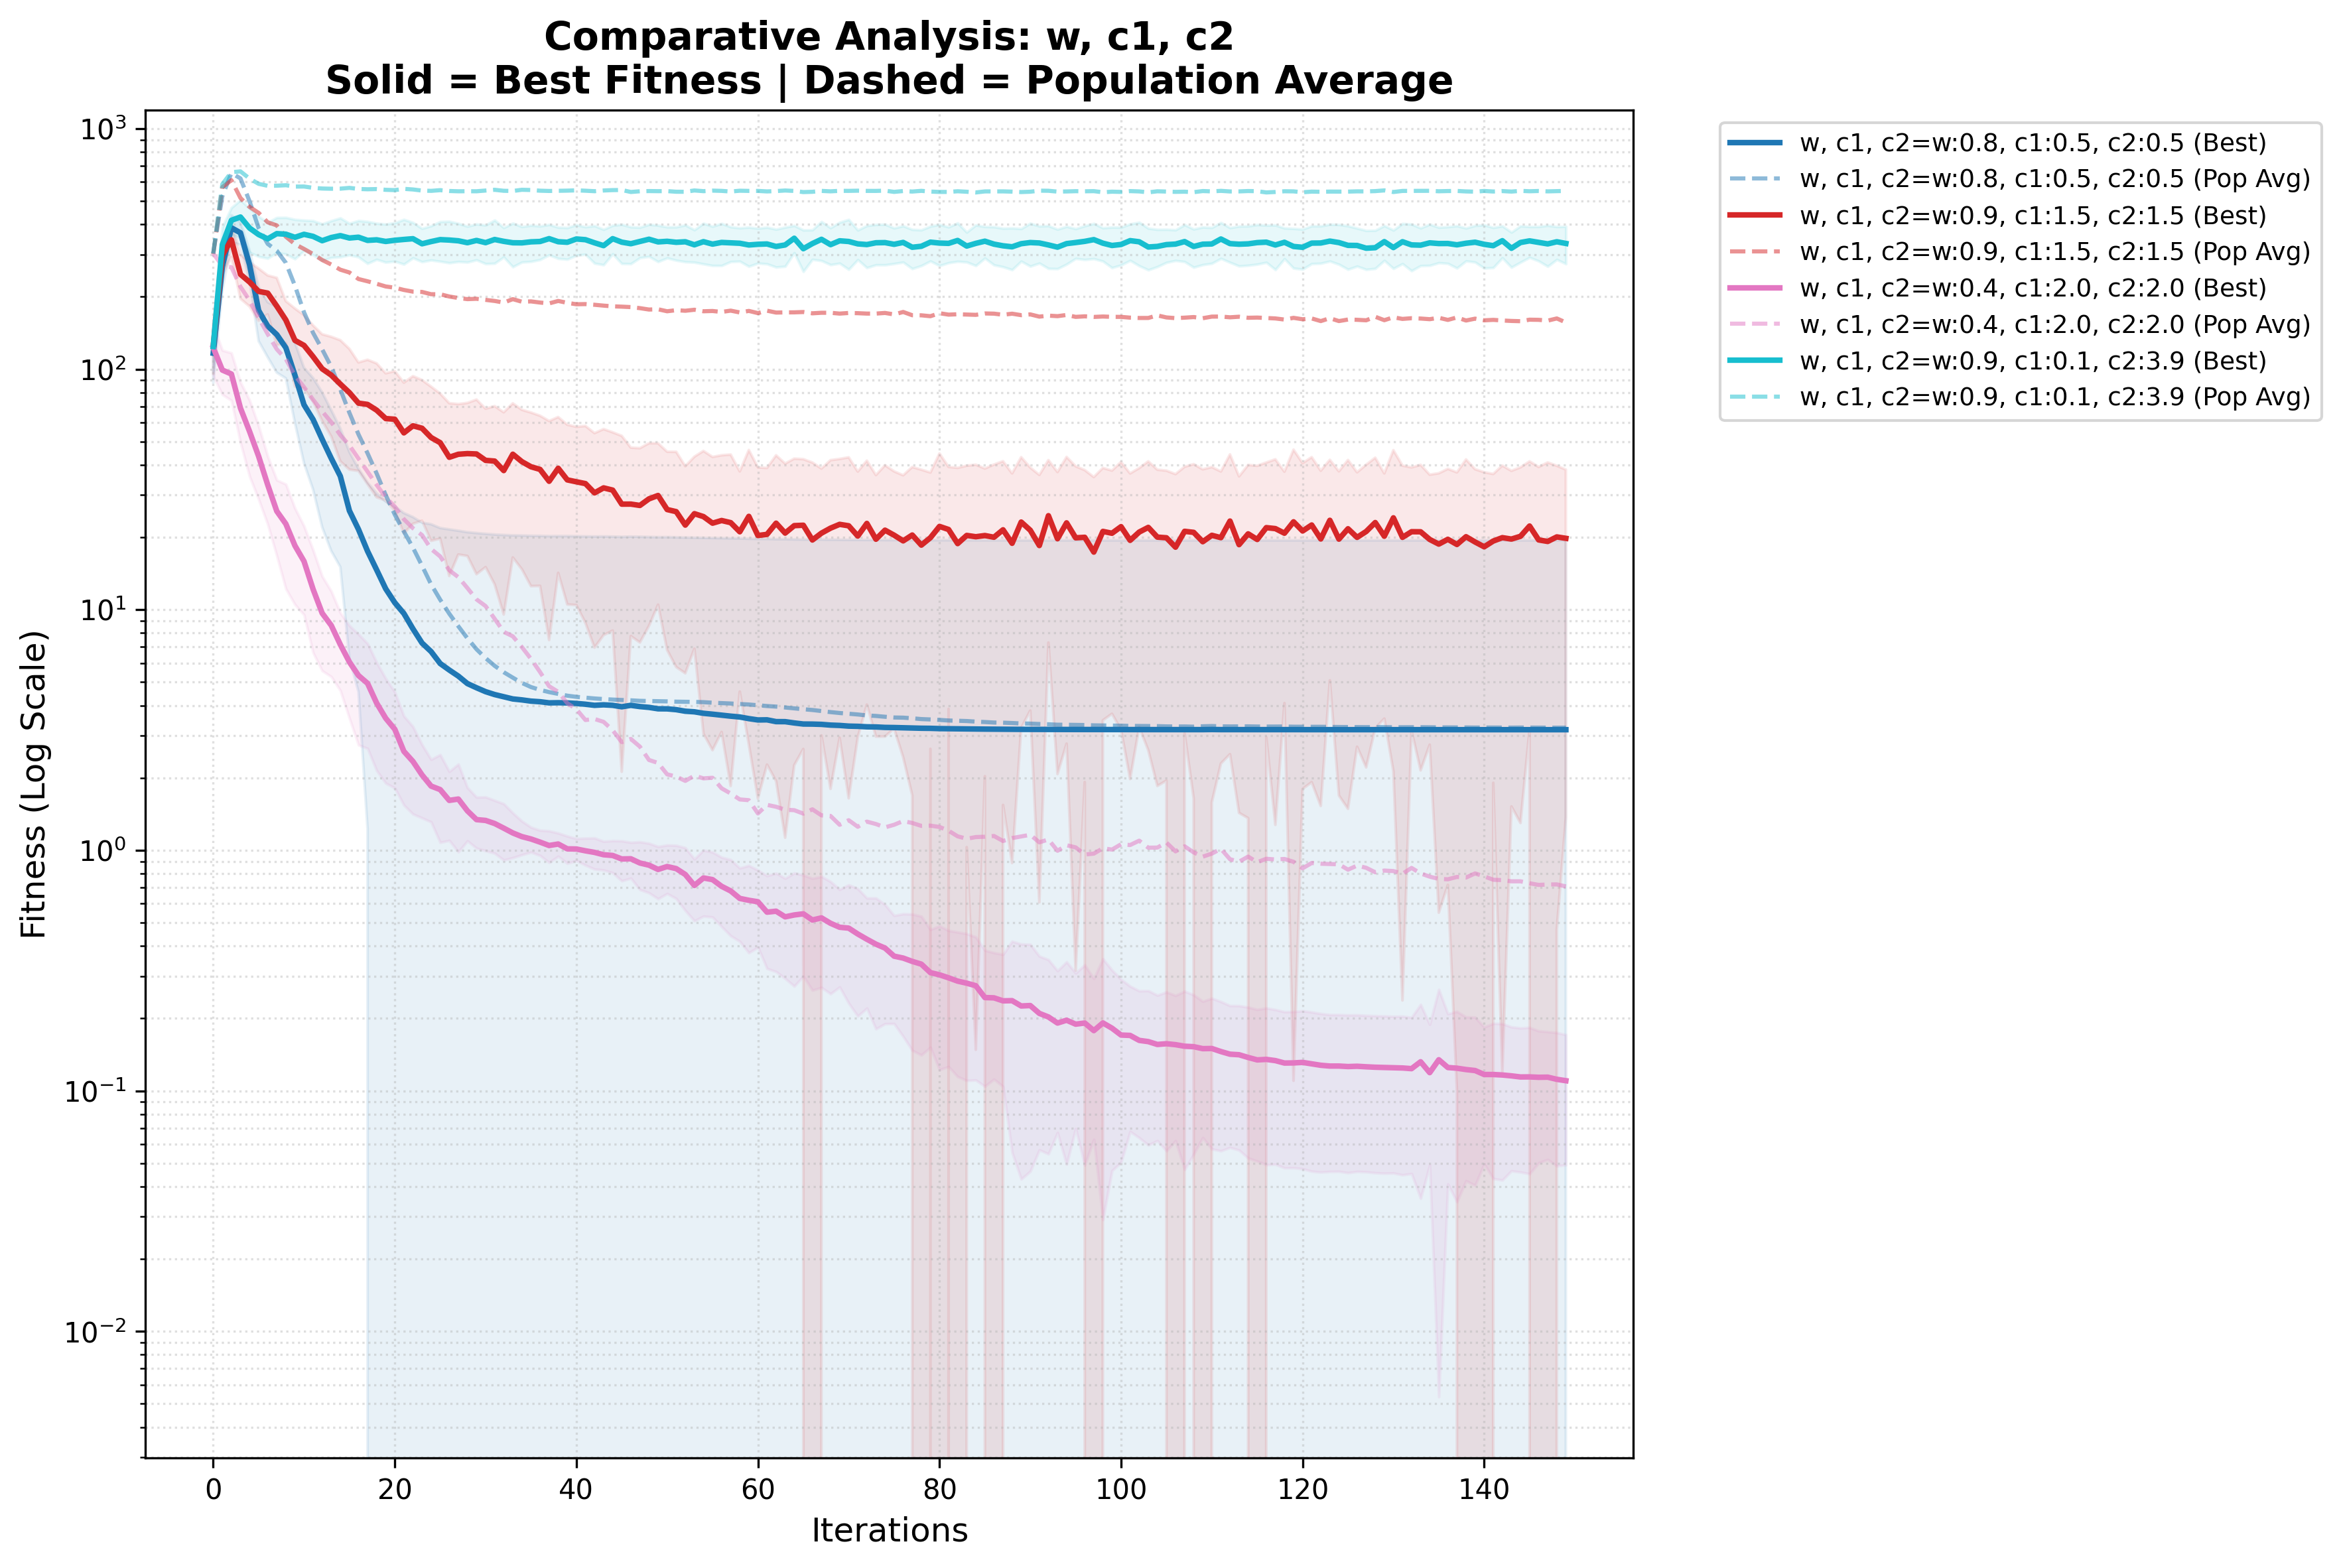
\includegraphics[width=1\linewidth]{comparativa_final_pso_griewank_w.png}
            \caption{Comparison of different w, c1 and c2 configurations on the Griewank function.}
            \label{fig:placeholder}
        \end{figure}
        
        In the solid lines we can appreciate the evolution of the best fitness, along with its standard deviation in the shaded area, while the dashed line represents the average of population average. 
        As we expected, this configuration was the fastest to converge, reaching a very low fitness already in the first 30 generations and still dropping steadily until the end. Additionally, we can apprecieta how it is the only
        combination that did not get stuck on a local minimum. This behaviour is explained by its overall equilibrium, the inertia weight of 0.4 allows the particles to maintain a good balance between exploration and exploitation, while the cognitive and social coefficients of 2.0 encourage the particles to effectively utilize both their own experience and the swarm's collective knowledge. 

        On the contrary, the worst configuration, the one with $w=0.9$, $c_1=0.1$ and $c_2=3.9$, shows a very erratic behaviour, with a very high standard deviation and a very slow convergence, which is explained by the fact that the particles are too social and not cognitive enough, they rely too much on the swarm's collective knowledge and not enough on their own experience, which can lead to premature convergence and getting stuck in local minimums, as we can see in the graph.

        Finally, the other two configurations, the moderate exploration and the high exploration, show a similar behaviour, with a slow convergence and a high standard deviation, which is explained by the fact that they have a high inertia weight, which allows the particles to explore more, but also makes them more likely to get stuck in local minimums as well.
    
        
         With this in mind, we decided to further explore the area around the winning configuration, testing the following values:
         
         \begin{table}[h!]
                \centering
                \begin{tabular}{c c c c l}
                \hline
                \textbf{Config} & \textbf{w} & \textbf{c1} & \textbf{c2} & \textbf{Description} \\
                \hline
                1 & 0.4 & 2.0 & 2.0 & Best initial configuration \\
                2 & 0.5 & 2.0 & 2.0 & Slightly higher inertia \\
                3 & 0.3 & 2.0 & 2.0 & Slightly lower inertia \\
                4 & 0.4 & 1.5 & 2.5 & More social, less cognitive ($c_1 + c_2 = 4$) \\
                5 & 0.4 & 2.5 & 1.5 & More cognitive, less social ($c_1 + c_2 = 4$) \\
                6 & 0.5 & 1.5 & 1.5 & Higher inertia, less social and cognitive ($c_1 + c_2 = 3$) \\
                \hline
                \end{tabular}
                \caption{Additional parameter configurations for fine-tuning around the best initial configuration.}
            \end{table}
        
       
        
            
            The results were the following: 

        \begin{table}[H]
        \centering
        \begin{tabular}{c c c c c c}
        \hline
        \textbf{w} & \textbf{c1} & \textbf{c2} & \textbf{Avg Fit} & \textbf{Min Fit} & \textbf{Std Dev} \\
        \hline
        0.4 & 2.0 & 2.0 & 0.128370 & 0.046725 & 0.069007 \\
        0.5 & 2.0 & 2.0 & 0.195165 & 0.020333 & 0.117131 \\
        0.3 & 2.0 & 2.0 & 0.110484 & 0.027086 & 0.072577 \\
        0.4 & 1.5 & 2.5 & 0.121947 & 0.026916 & 0.077329 \\
        0.4 & 2.5 & 1.5 & 0.094049 & 0.029510 & 0.043736 \\
        0.5 & 1.5 & 1.5 & 0.100378 & 0.019678 & 0.060535 \\
        \hline
        \end{tabular}
        \caption{Definitive results of w, c1 and c2 on PSO, 10-dimensional Griewank function.}
        \end{table}
        In this case, the results were remarkably similar, as their behaviour is considerably mor similar than before. Nonetheless, the configuration considered to be the best is the one with $w=0.4$, $c_1=2.5$ and $c_2=1.5$, as it is the most stable, achieving the best average fitness and standard deviation, while maintaining a good minimum fitness. 
        The key of this success relies on the importance given to the cognitive component (as it is the only difference between the previous best), in Griewank we have a high quantity of local minimums, 
        so you want particles to behave more independently at first, instead of blindly following the current global best because if at the beggining we start to give more importance to the social component, all particles will be attracted to the same local minimum, and it will be very hard for them to escape from it, while if we give more importance to the cognitive component, particles will have more freedom to explore the search space and find better solutions, even if they are not the current global best.
        
        The comparative graph gives more information:
        \begin{figure}[H]
            \centering
            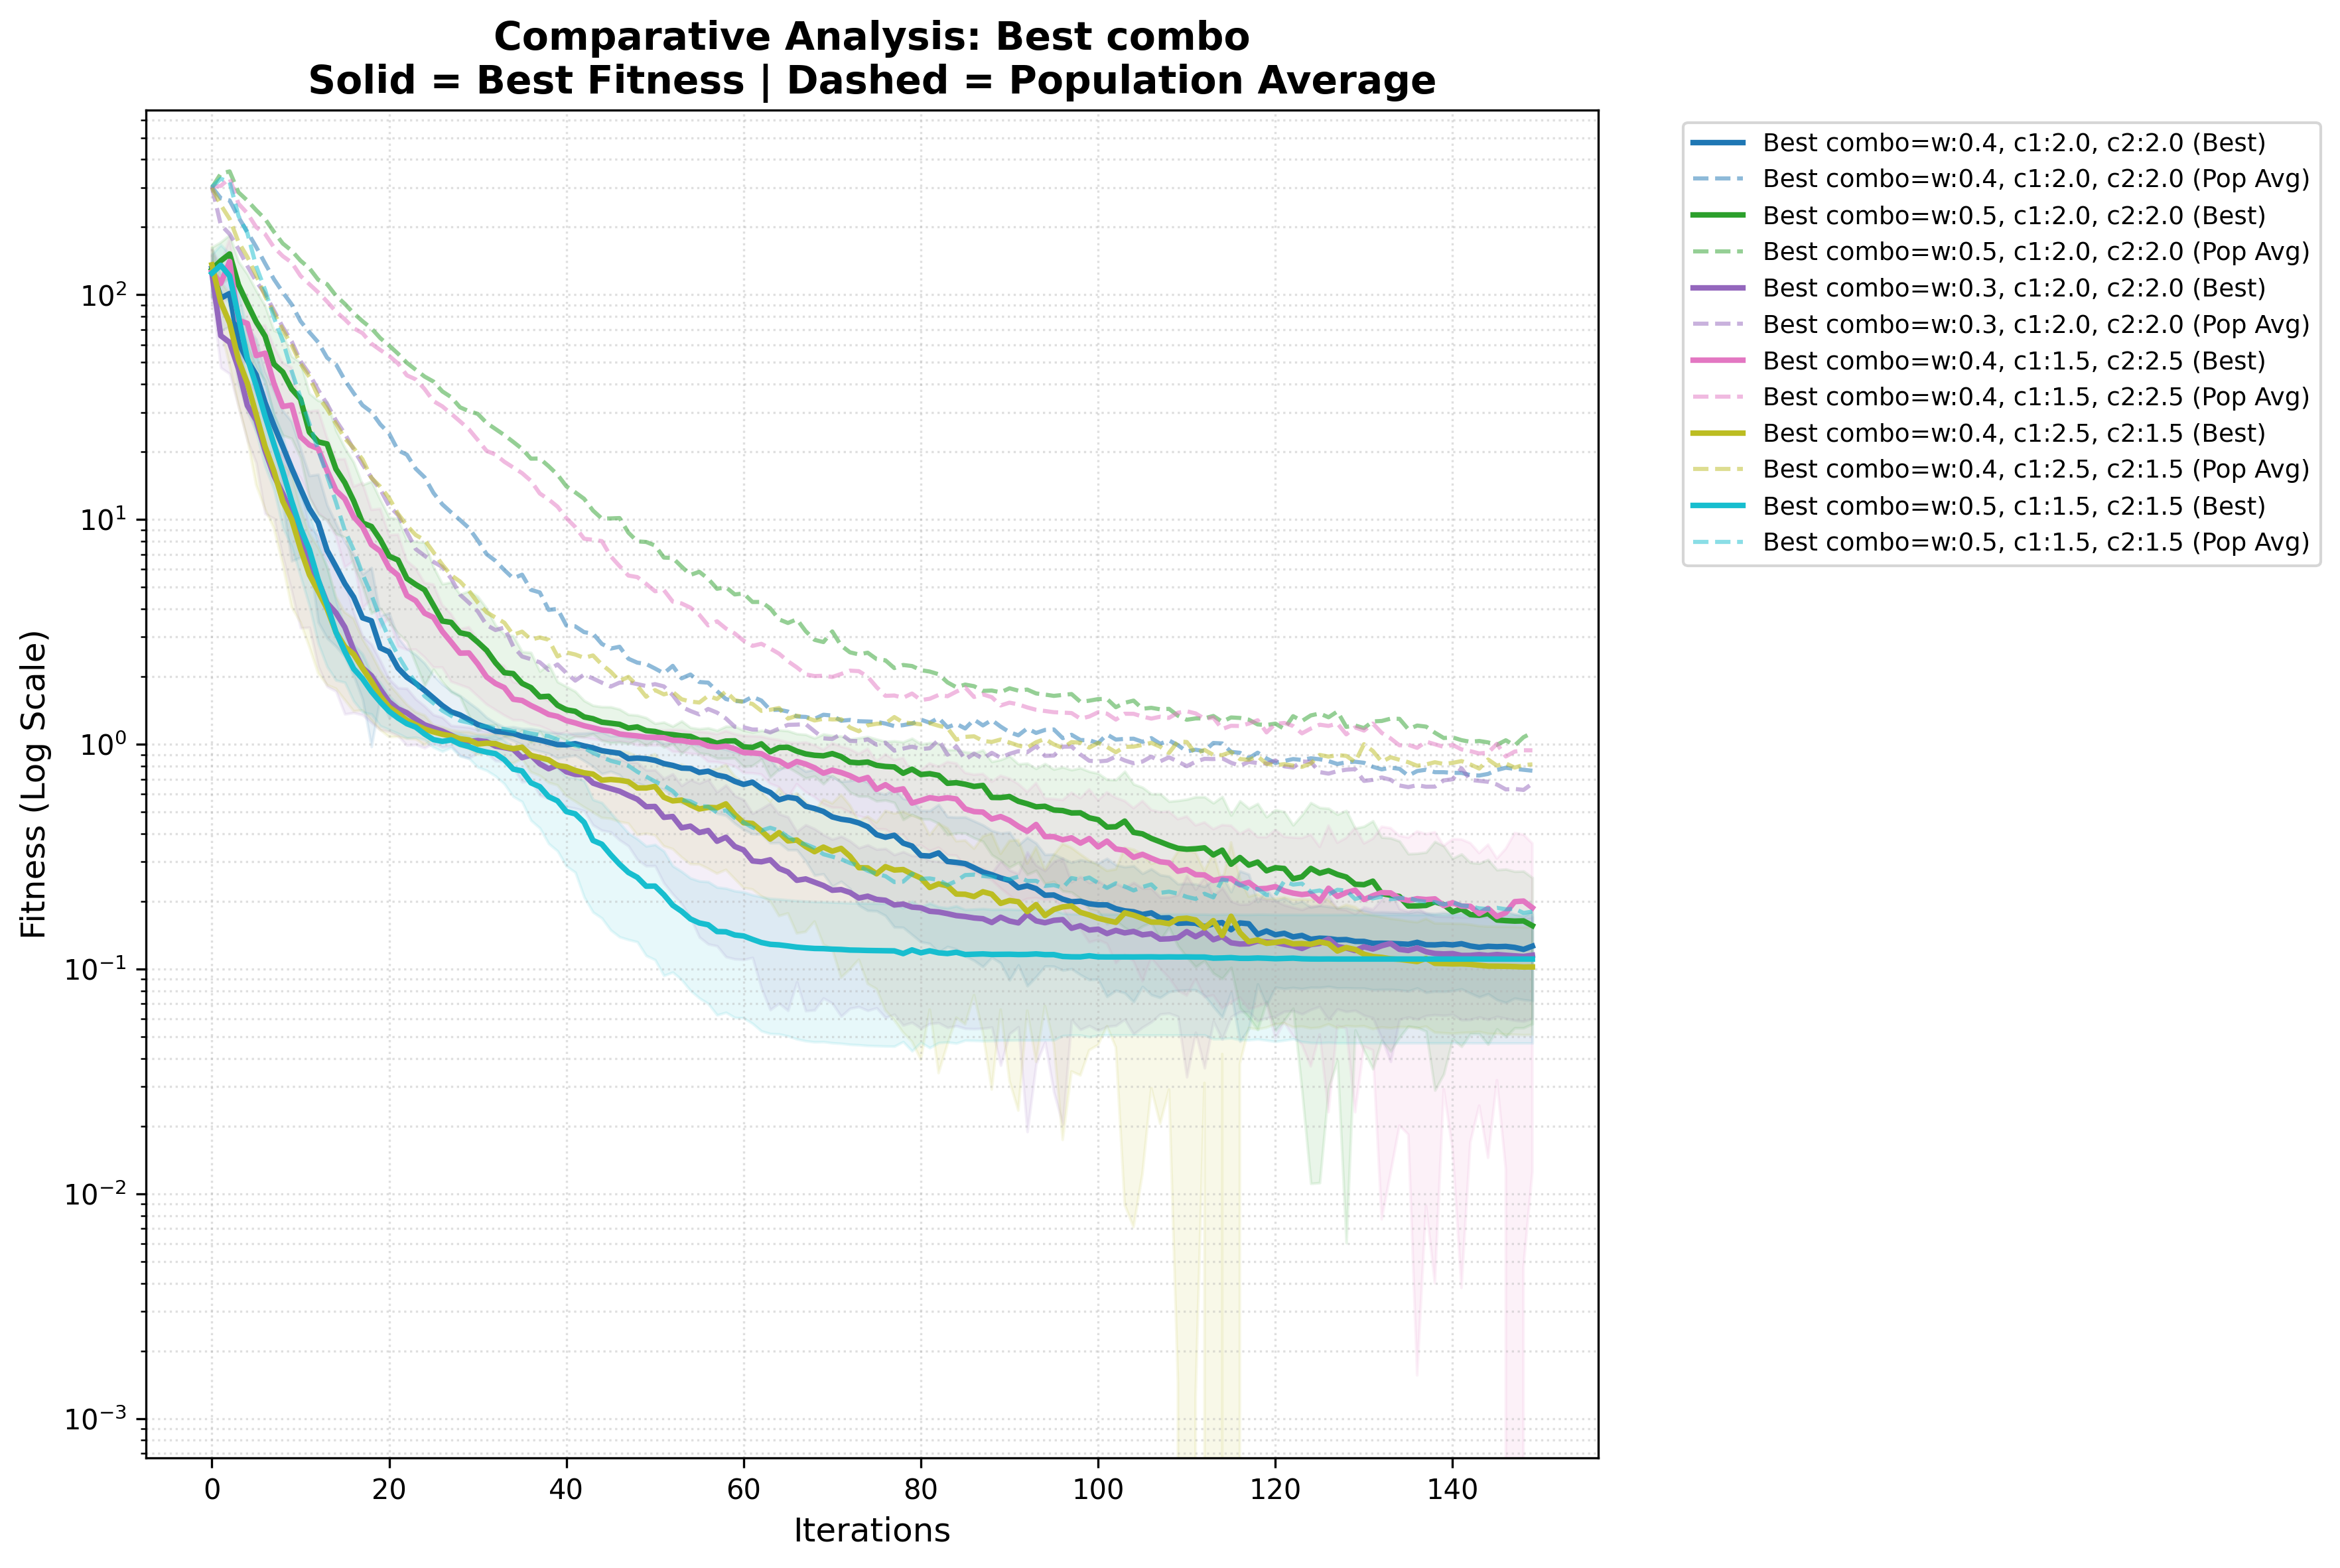
\includegraphics[width=1\linewidth]{comparativa_final_pso_griewank_w_expanded.png}
            \caption{Comparison of the best configuration with other similar configurations.}
            \label{fig:placeholder}
        \end{figure}

        As we expected, the new best configuration (yellow), while not being the first to reach a low fitness, it is the winner at the end of the iterations. 
            
        \item \textbf{Population}
        
        Once we had the best configuration of $w$, $c_1$ and $c_2$, we decided to test the impact of the population size, testing the following values: 30, 50, 200 and 600. These values were chosen to represent a low population (30, 50), a medium population (200) and a high population (600) and test the behaviour on these three scenarios. The results were the following:
        \begin{table}[H]
        \centering
        \begin{tabular}{c c c c}
        \hline
        Population & Avg Fit & Min Fit & Std Dev \\
        \hline
        30  & 0.128553 & 0.009866 & 0.067793 \\
        50  & 0.111909 & 0.024644 & 0.070827 \\
        200 & 0.076620 & 0.016973 & 0.032238 \\
        600 & 0.072795 & 0.019693 & 0.024755 \\
        \hline
        \end{tabular}
        \caption{Results PSO – Griewank 10D}
        \end{table}
        These are not shocking, because as we know, increasing the population size generally leads to better performance in optimization algorithms, as it allows for a more diverse search of the solution space and reduces the chances of getting stuck in local minimums.
        In this case, we can see that as the population size increases, the average fitness improves (decreases) and the standard deviation decreases as well, indicating that the algorithm is finding better solutions more consistently. The minimum fitness also improves with larger populations, which suggests that the algorithm is able to find better solutions overall.
        \begin{figure}[H]
            \centering
            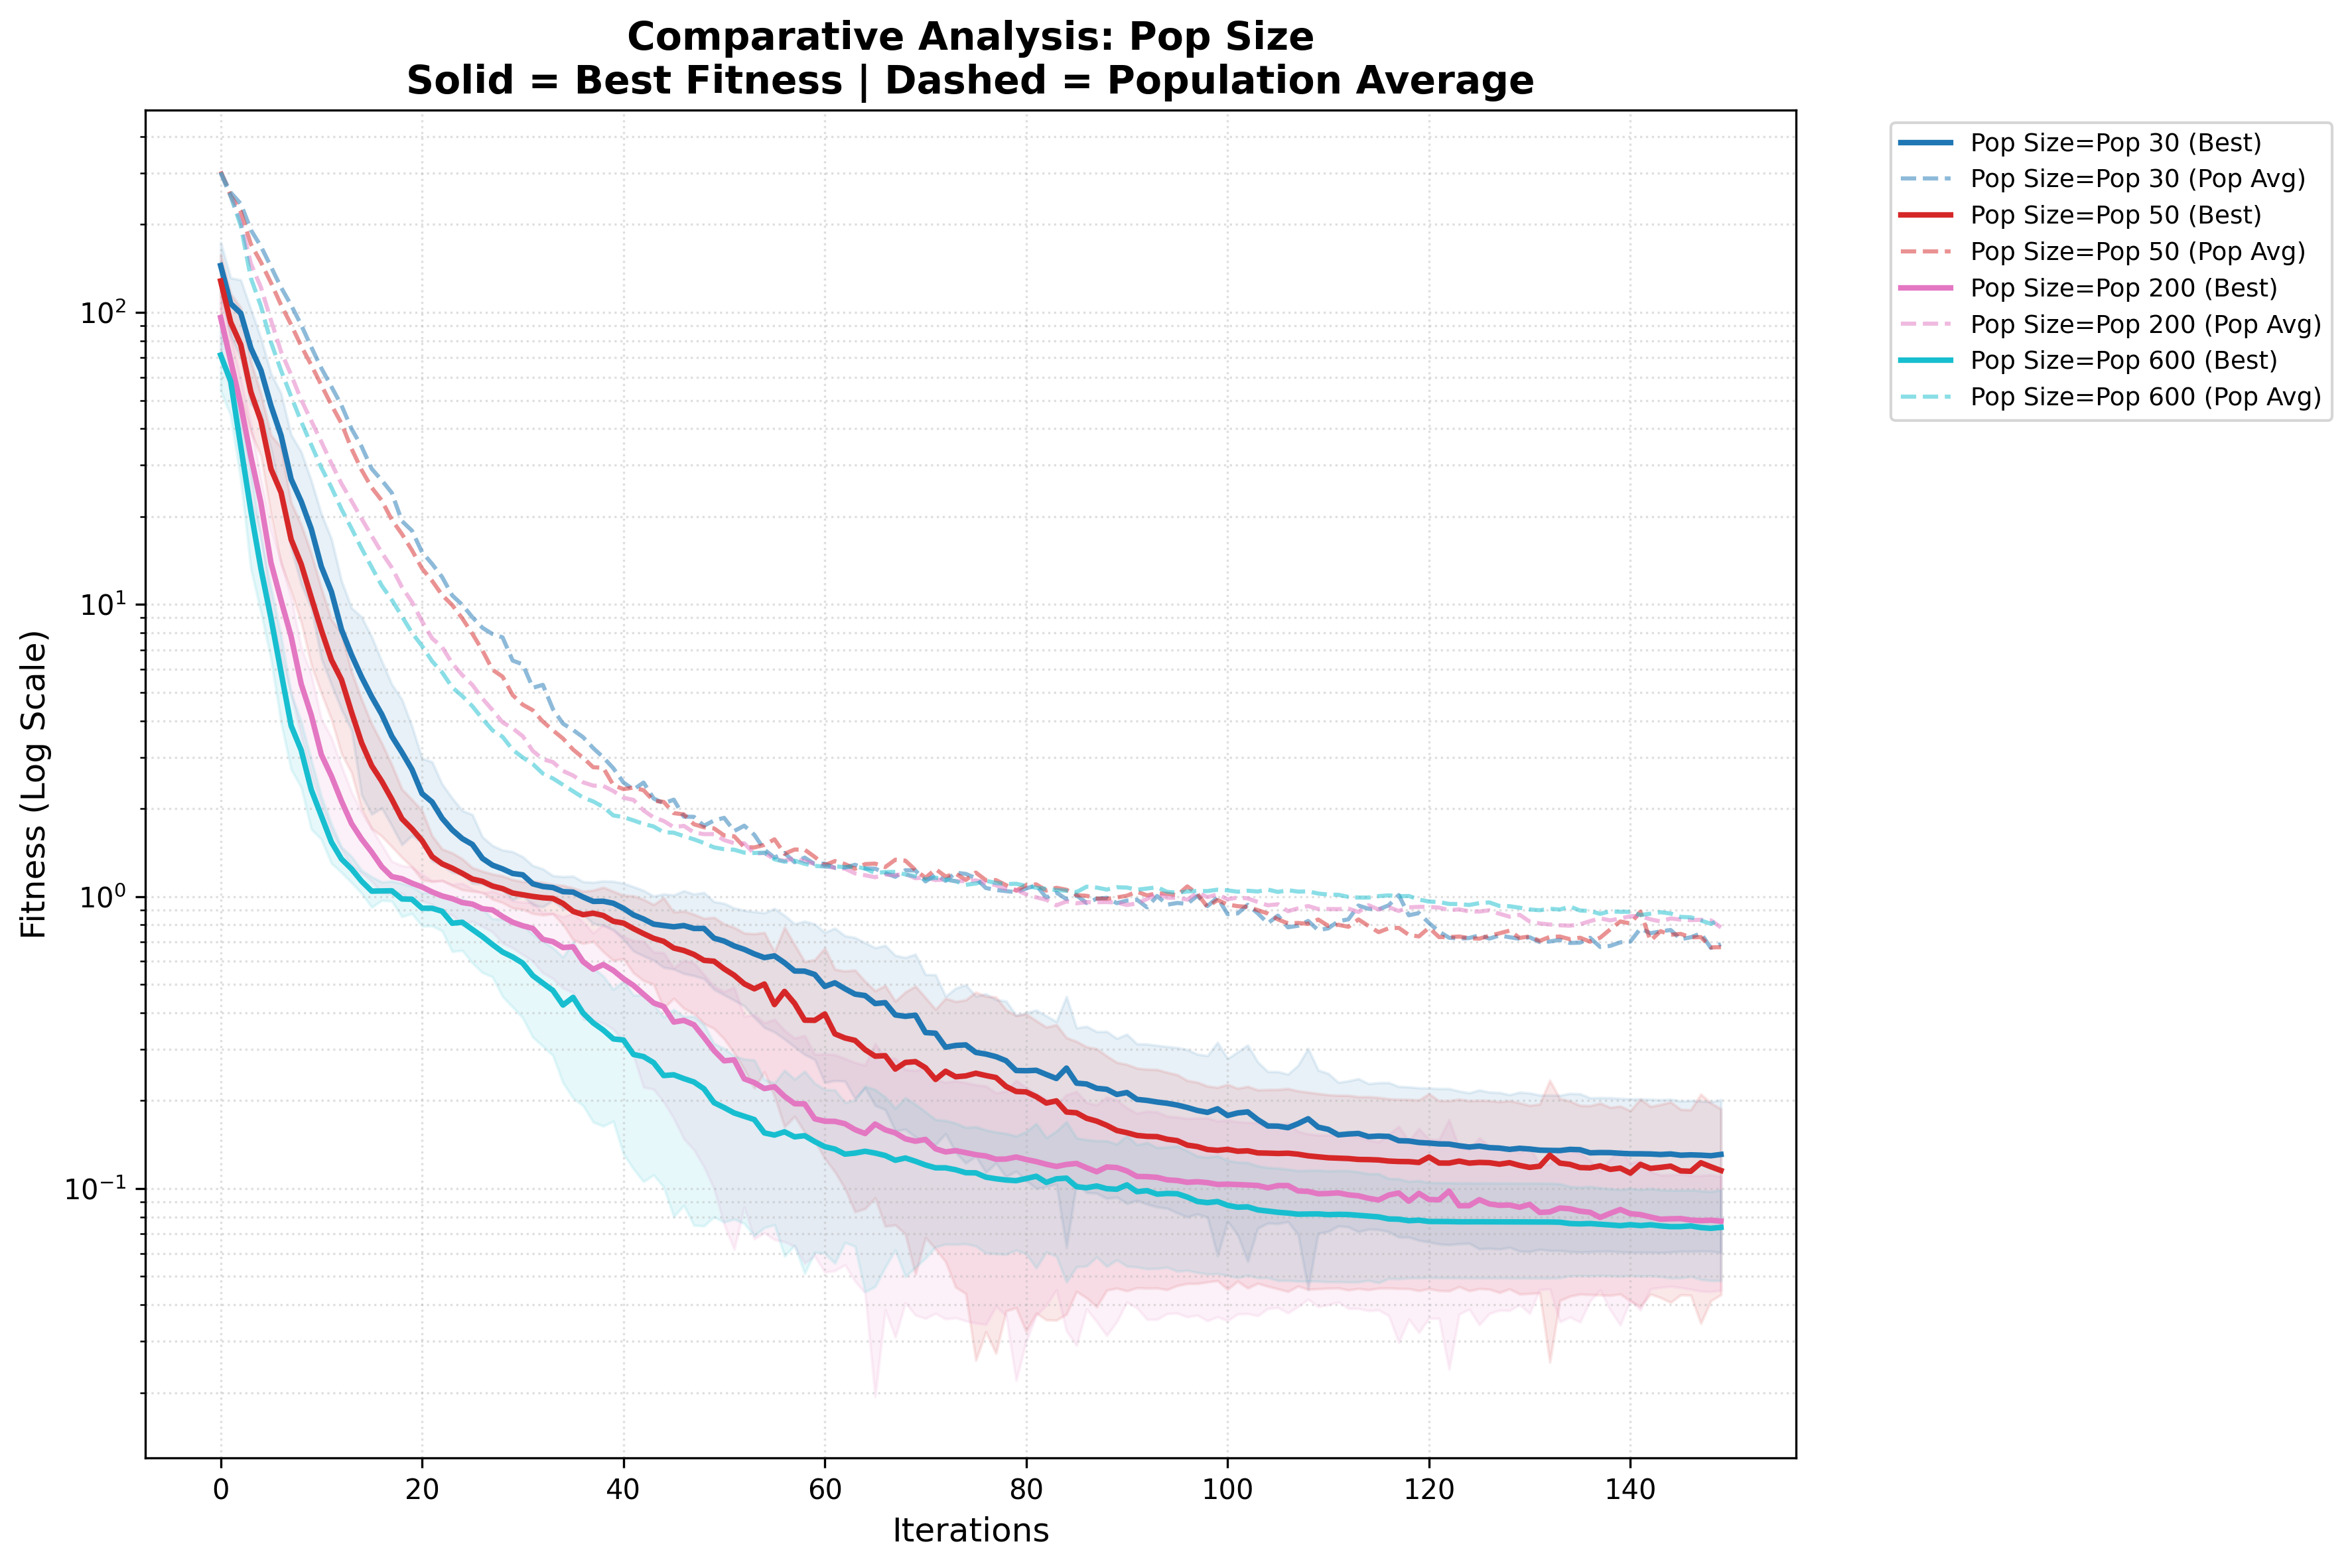
\includegraphics[width=1\linewidth]{comparativa_final_pso_griewank_pop.png}
            \caption{Results of the experiments based on population}
            \label{fig:placeholder}
        \end{figure}
        In the graph we can see, how with 600 individuals, the algorithm converges faster but at the same time, its average of population average does not improve in comparison to the other population sizes. This phenomenon may be because with a larger population, the algorithm is able to find good solutions faster, but it may also be more likely to get stuck in local minimums, 
        because a large population reduces diversity too quickly. Therefore the large part of the swarm that get stuck in the minimums affect the population average, while the best fitness can still improve because of the few individuals that are able to escape from those minimums.


        \item \textbf{Number of Iterations}
        
        Finally, we tested the impact of the number of iterations, we used the same criteria as before with three values to represent a low, medium and high number of iterations.
        We are aware that this variable will only give more "time" to the algorithm to find better solutions, but we wanted to test if there was a point of diminishing returns, where increasing the number of iterations does not lead to significant improvements in fitness or if, on the contrary, there's a threshold of iterations needed to drastically improve the results. The results were the following:
        \begin{table}[h!]
        \centering
        \begin{tabular}{c c c c}
        \hline
        Iterations & Avg Fit & Min Fit & Std Dev \\
        \hline
        150 & 0.078052 & 0.032296 & 0.043496 \\
        300 & 0.059282 & 0.014780 & 0.028738 \\
        600 & 0.047147 & 0.014772 & 0.020200 \\
        \hline
        \end{tabular}
        \caption{Results PSO – Griewank 10D}
        \end{table}

        \begin{figure}[H]
            \centering
            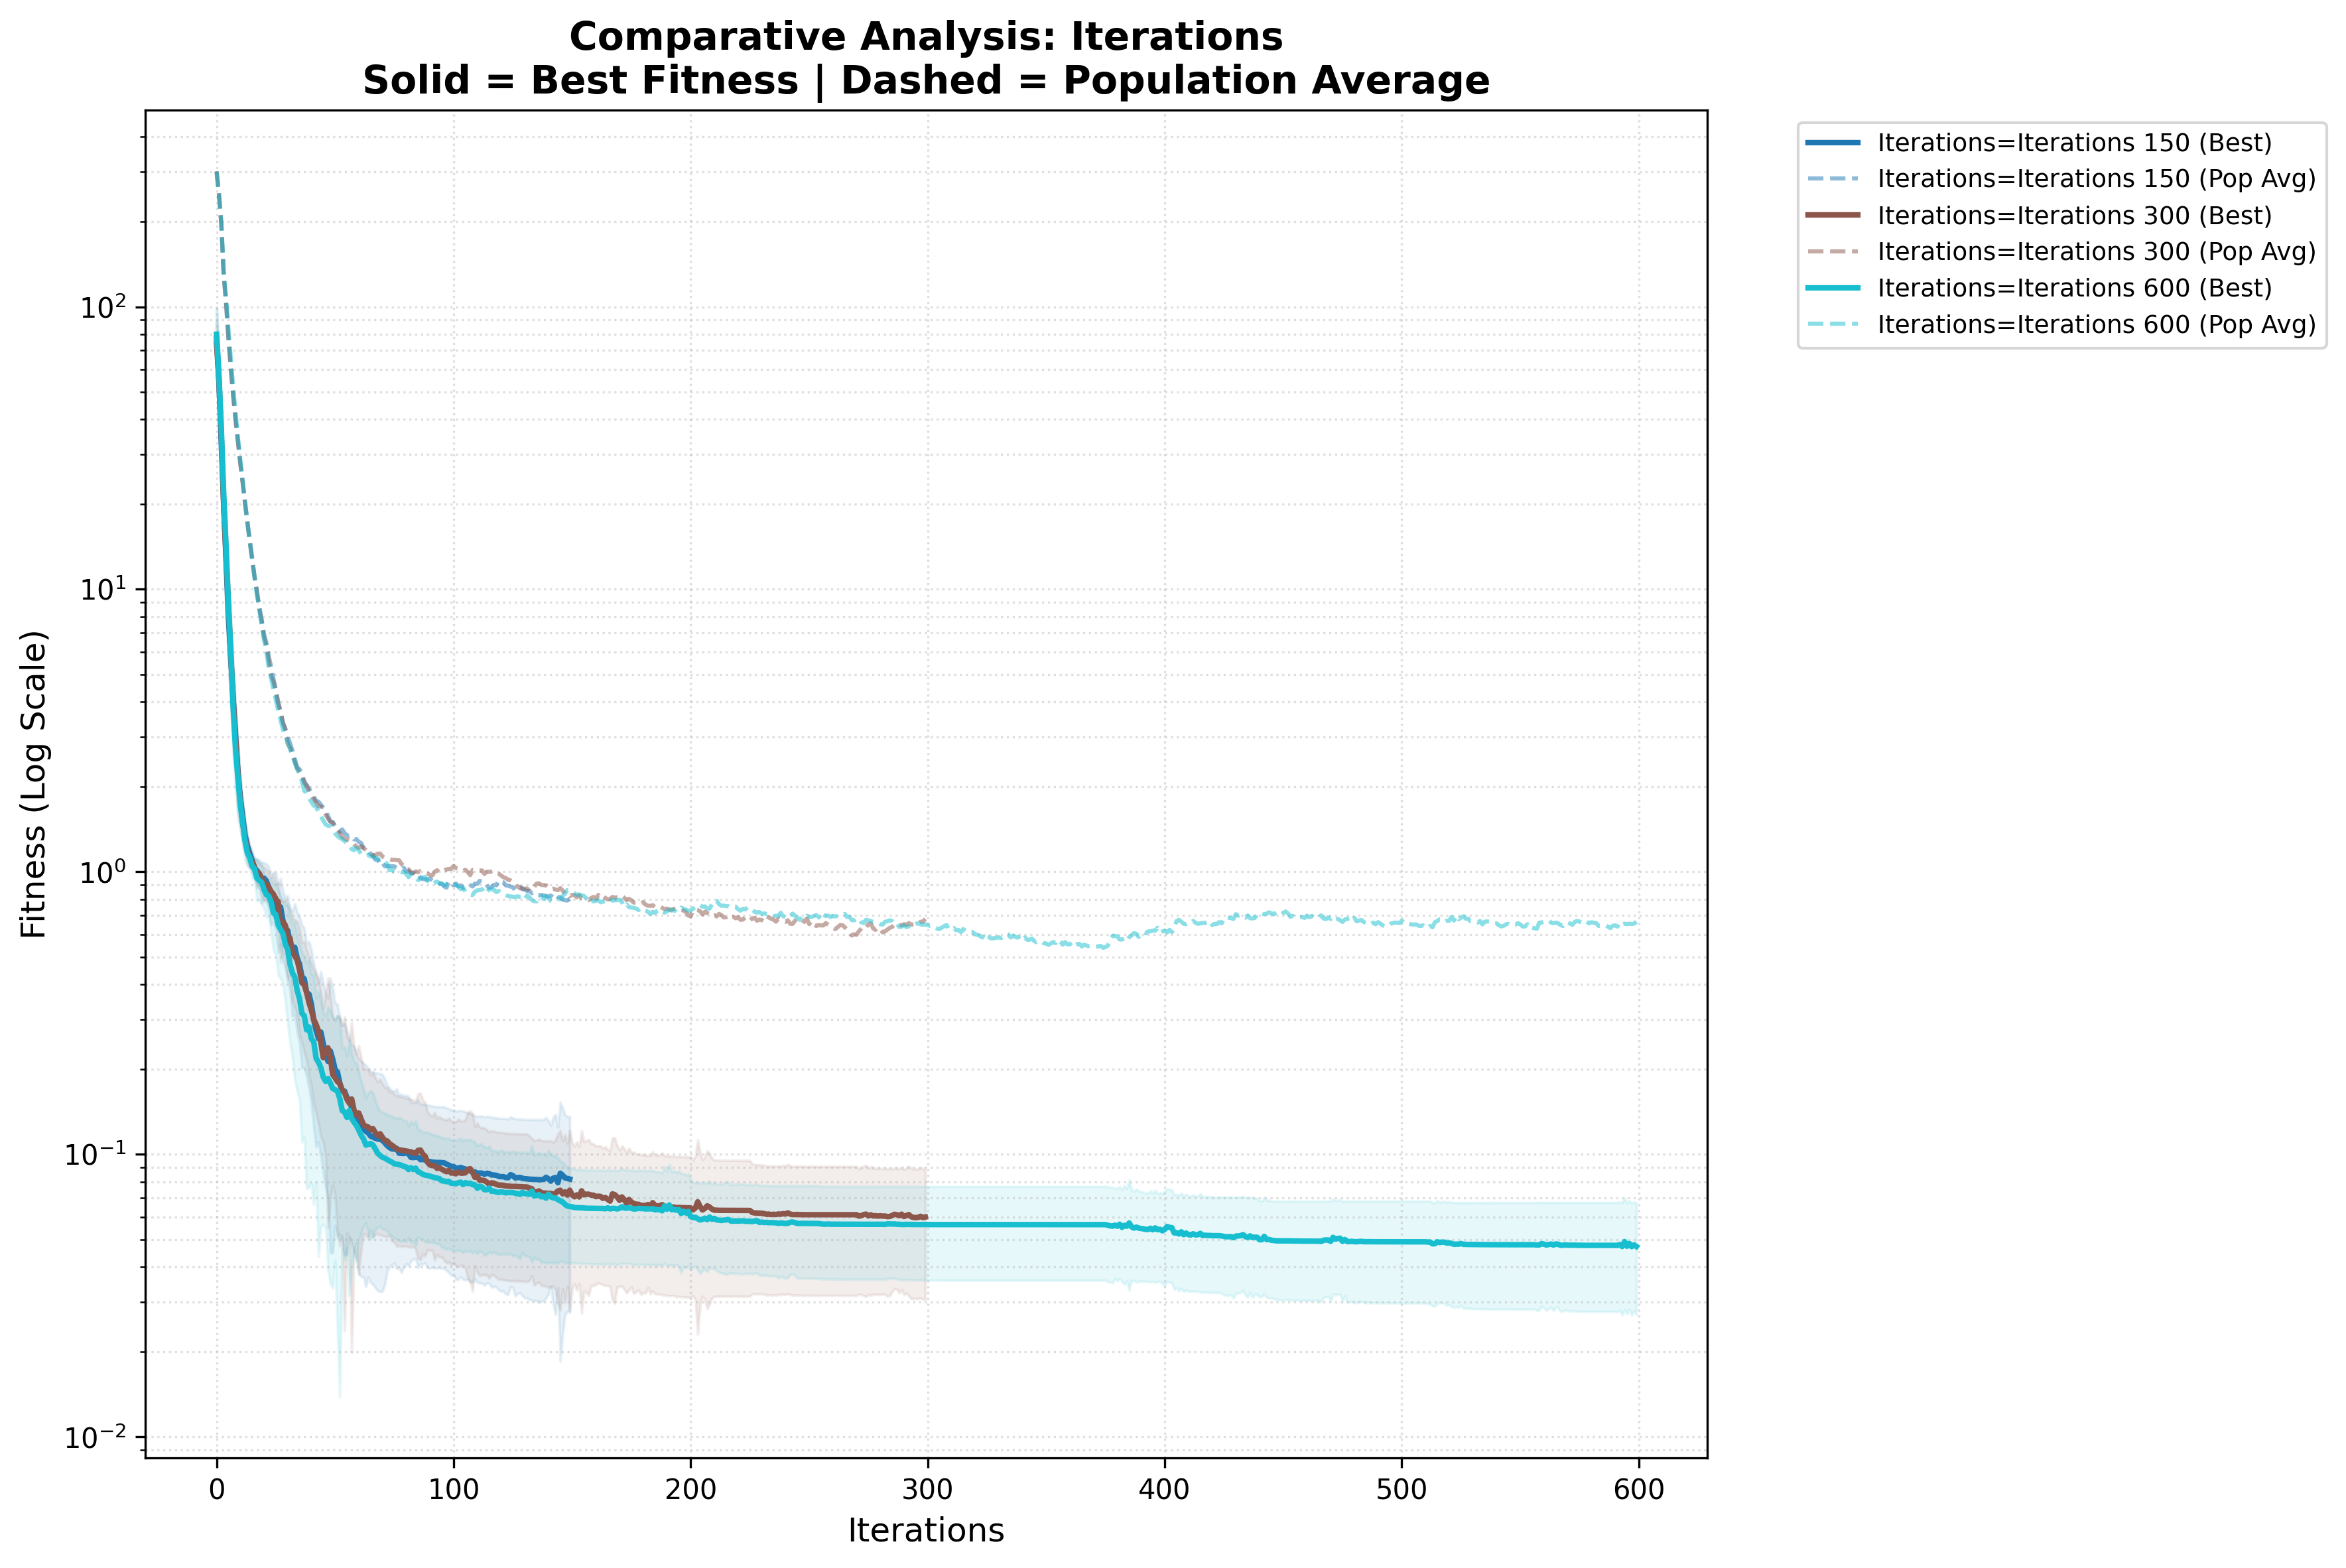
\includegraphics[width=1\linewidth]{comparativa_final_pso_griewank_iterations.png}
            \caption{Results of the experiments based on population}
            \label{fig:placeholder}
        \end{figure}
        We can appreciate how in this specific scenario, there's a significant improvement when going from low to medium iterations, but from that point on the improvements become less relevant. This can be attributable to the Griewank function's multimodal landscape: once the swarm has identified a reasonably good basin of attraction, additional iterations tend to refine the solution only marginally. The particles gradually lose diversity as they are pulled toward the same region, so the algorithm’s ability to escape to a better basin diminishes.
    \end{itemize}    
        
\subsubsection{Rosenbrock function with PSO}

In this section, we will repeat the same experiments as with the Griewank section, but with Rosenbrock as fitness function. 
All the values of the variables were the same as before, except for the domain, which was set to the range of [-5, 5] and of course the best w, c1 and c2, which will be determined.
\paragraph{Discussion of Results}
\begin{itemize} 
        \item \textbf{w, c1 and c2}
        
        The results of the configurations were the following:
        \begin{table}[H]
        \centering
        \begin{tabular}{c c c c c c}
        \hline
        $w$ & $c_1$ & $c_2$ & Avg Fit & Min Fit & Std Dev \\
        \hline
        0.8 & 0.5 & 0.5 & 203.828906 & 1.835968 & 461.019983 \\
        0.9 & 1.5 & 1.5 & 654.842261 & 64.689540 & 911.626978 \\
        0.4 & 2.0 & 2.0 & 9.636683 & 0.187247 & 16.723237 \\
        0.9 & 0.1 & 3.9 & 90075.129604 & 48315.587328 & 33616.773437 \\
        \hline
        \end{tabular}
        \caption{Results PSO – Rosenbrock 10D}
        \end{table}

        We can appreciate how, again, the winning configuration is the one with $w=0.4$, $c_1=2.0$ and $c_2=2.0$, thanks to its balanced nature of exploration and exploitation and cognitive and social components. Here, the results are remarkably worse than in the Griewank function, which is explained by high difficulty of the Rosenbrock function,
         also the difference between the best and the worst configuration is much higher, which is as well explained by Rosenbrock's nature, which is a unimodal function with a narrow, parabolic-shaped valley. The high inertia weight and low cognitive/social coefficients in the worst configuration likely caused the particles to explore too broadly 
         and even fall outside the narrow valley, while the lower inertia of the winner seems to have been able to manage the steepness of the valley.
        \begin{figure}[H]
            \centering
            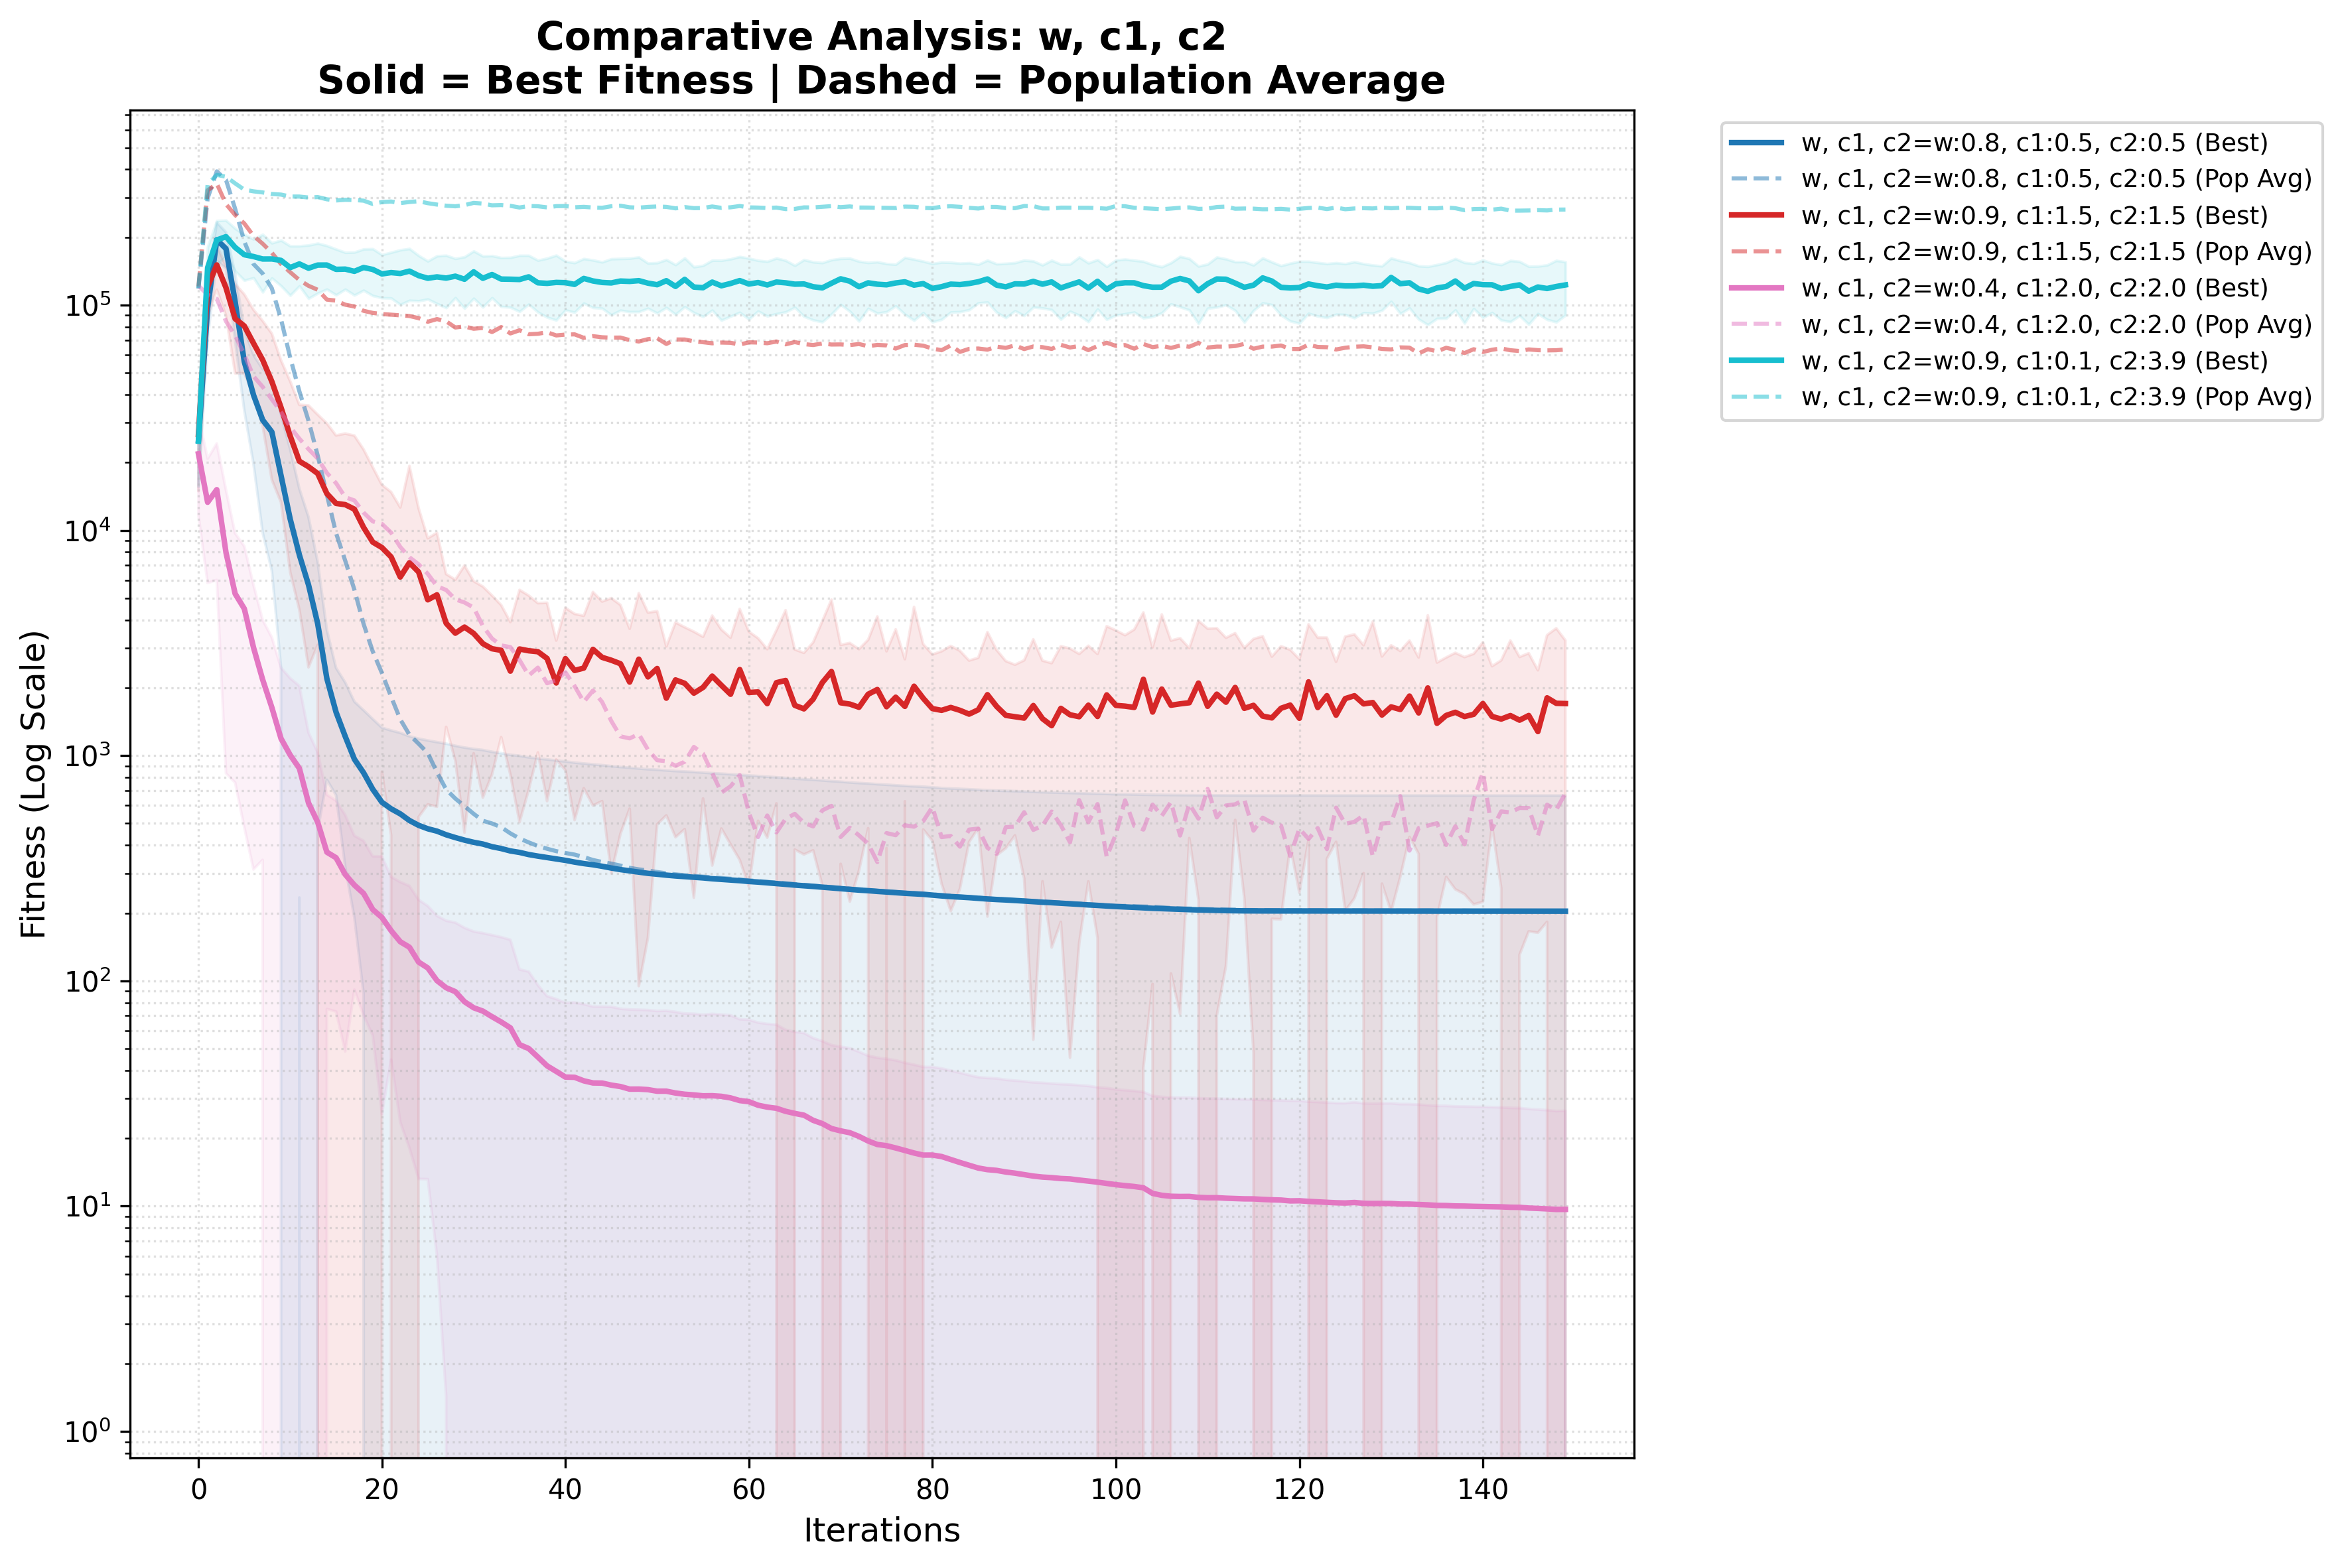
\includegraphics[width=1\linewidth]{comparativa_final_pso_rosenbrock_w.png}
            \caption{Enter Caption}
            \label{fig:placeholder}
        \end{figure}
        
        The plot gives more credibility to our hypothesis, as we can observe how the higher the inertia, the earlier the algorithm gets stuck in some local minimum. The lower inertia, on the other hand, allows the algorithm to keep exploring for a longer time, as we can see on the best configuration.
            
        Now, based on these findings, we tested the following configurations around the winner:
         \begin{table}[H]
                \centering
                \begin{tabular}{c c c c l}
                \hline
                \textbf{Config} & \textbf{w} & \textbf{c1} & \textbf{c2} & \textbf{Description} \\
                \hline
                1 & 0.4 & 2.0 & 2.0 & Best initial configuration \\
                2 & 0.5 & 2.0 & 2.0 & Slightly higher inertia \\
                3 & 0.3 & 2.0 & 2.0 & Slightly lower inertia \\
                4 & 0.4 & 1.5 & 2.5 & More social, less cognitive ($c_1 + c_2 = 4$) \\
                5 & 0.4 & 2.5 & 1.5 & More cognitive, less social ($c_1 + c_2 = 4$) \\
                6 & 0.5 & 1.5 & 1.5 & Higher inertia, less social and cognitive ($c_1 + c_2 = 3$) \\
                \hline
                \end{tabular}
                \caption{Additional parameter configurations for fine-tuning around the best initial configuration.}
        \end{table}
        
        And the results were the following:
        \begin{table}[H]
        \centering
        \begin{tabular}{c c c c c c}
        \hline
        \textbf{w} & \textbf{c1} & \textbf{c2} & \textbf{Avg Fit} & \textbf{Min Fit} & \textbf{Std Dev} \\
        \hline
        0.4 & 2.0 & 2.0 & 5.652720 & 1.835969 & 1.645278 \\
        0.5 & 2.0 & 2.0 & 30.541155 & 1.682337 & 89.561074 \\
        0.3 & 2.0 & 2.0 & 5.298981 & 0.114563 & 2.339122 \\
        0.4 & 1.5 & 2.5 & 22.868898 & 0.254218 & 45.768945 \\
        0.4 & 2.5 & 1.5 & 5.797184 & 3.161424 & 1.858188 \\
        0.5 & 1.5 & 1.5 & 114.799815 & 0.269950 & 454.250480 \\
        \hline
        \end{tabular}
        \caption{Definitive results of w, c1 and c2 on PSO, 10-dimensional Rosenbrock function.}
        \end{table}

        \begin{figure}[H]
            \centering
            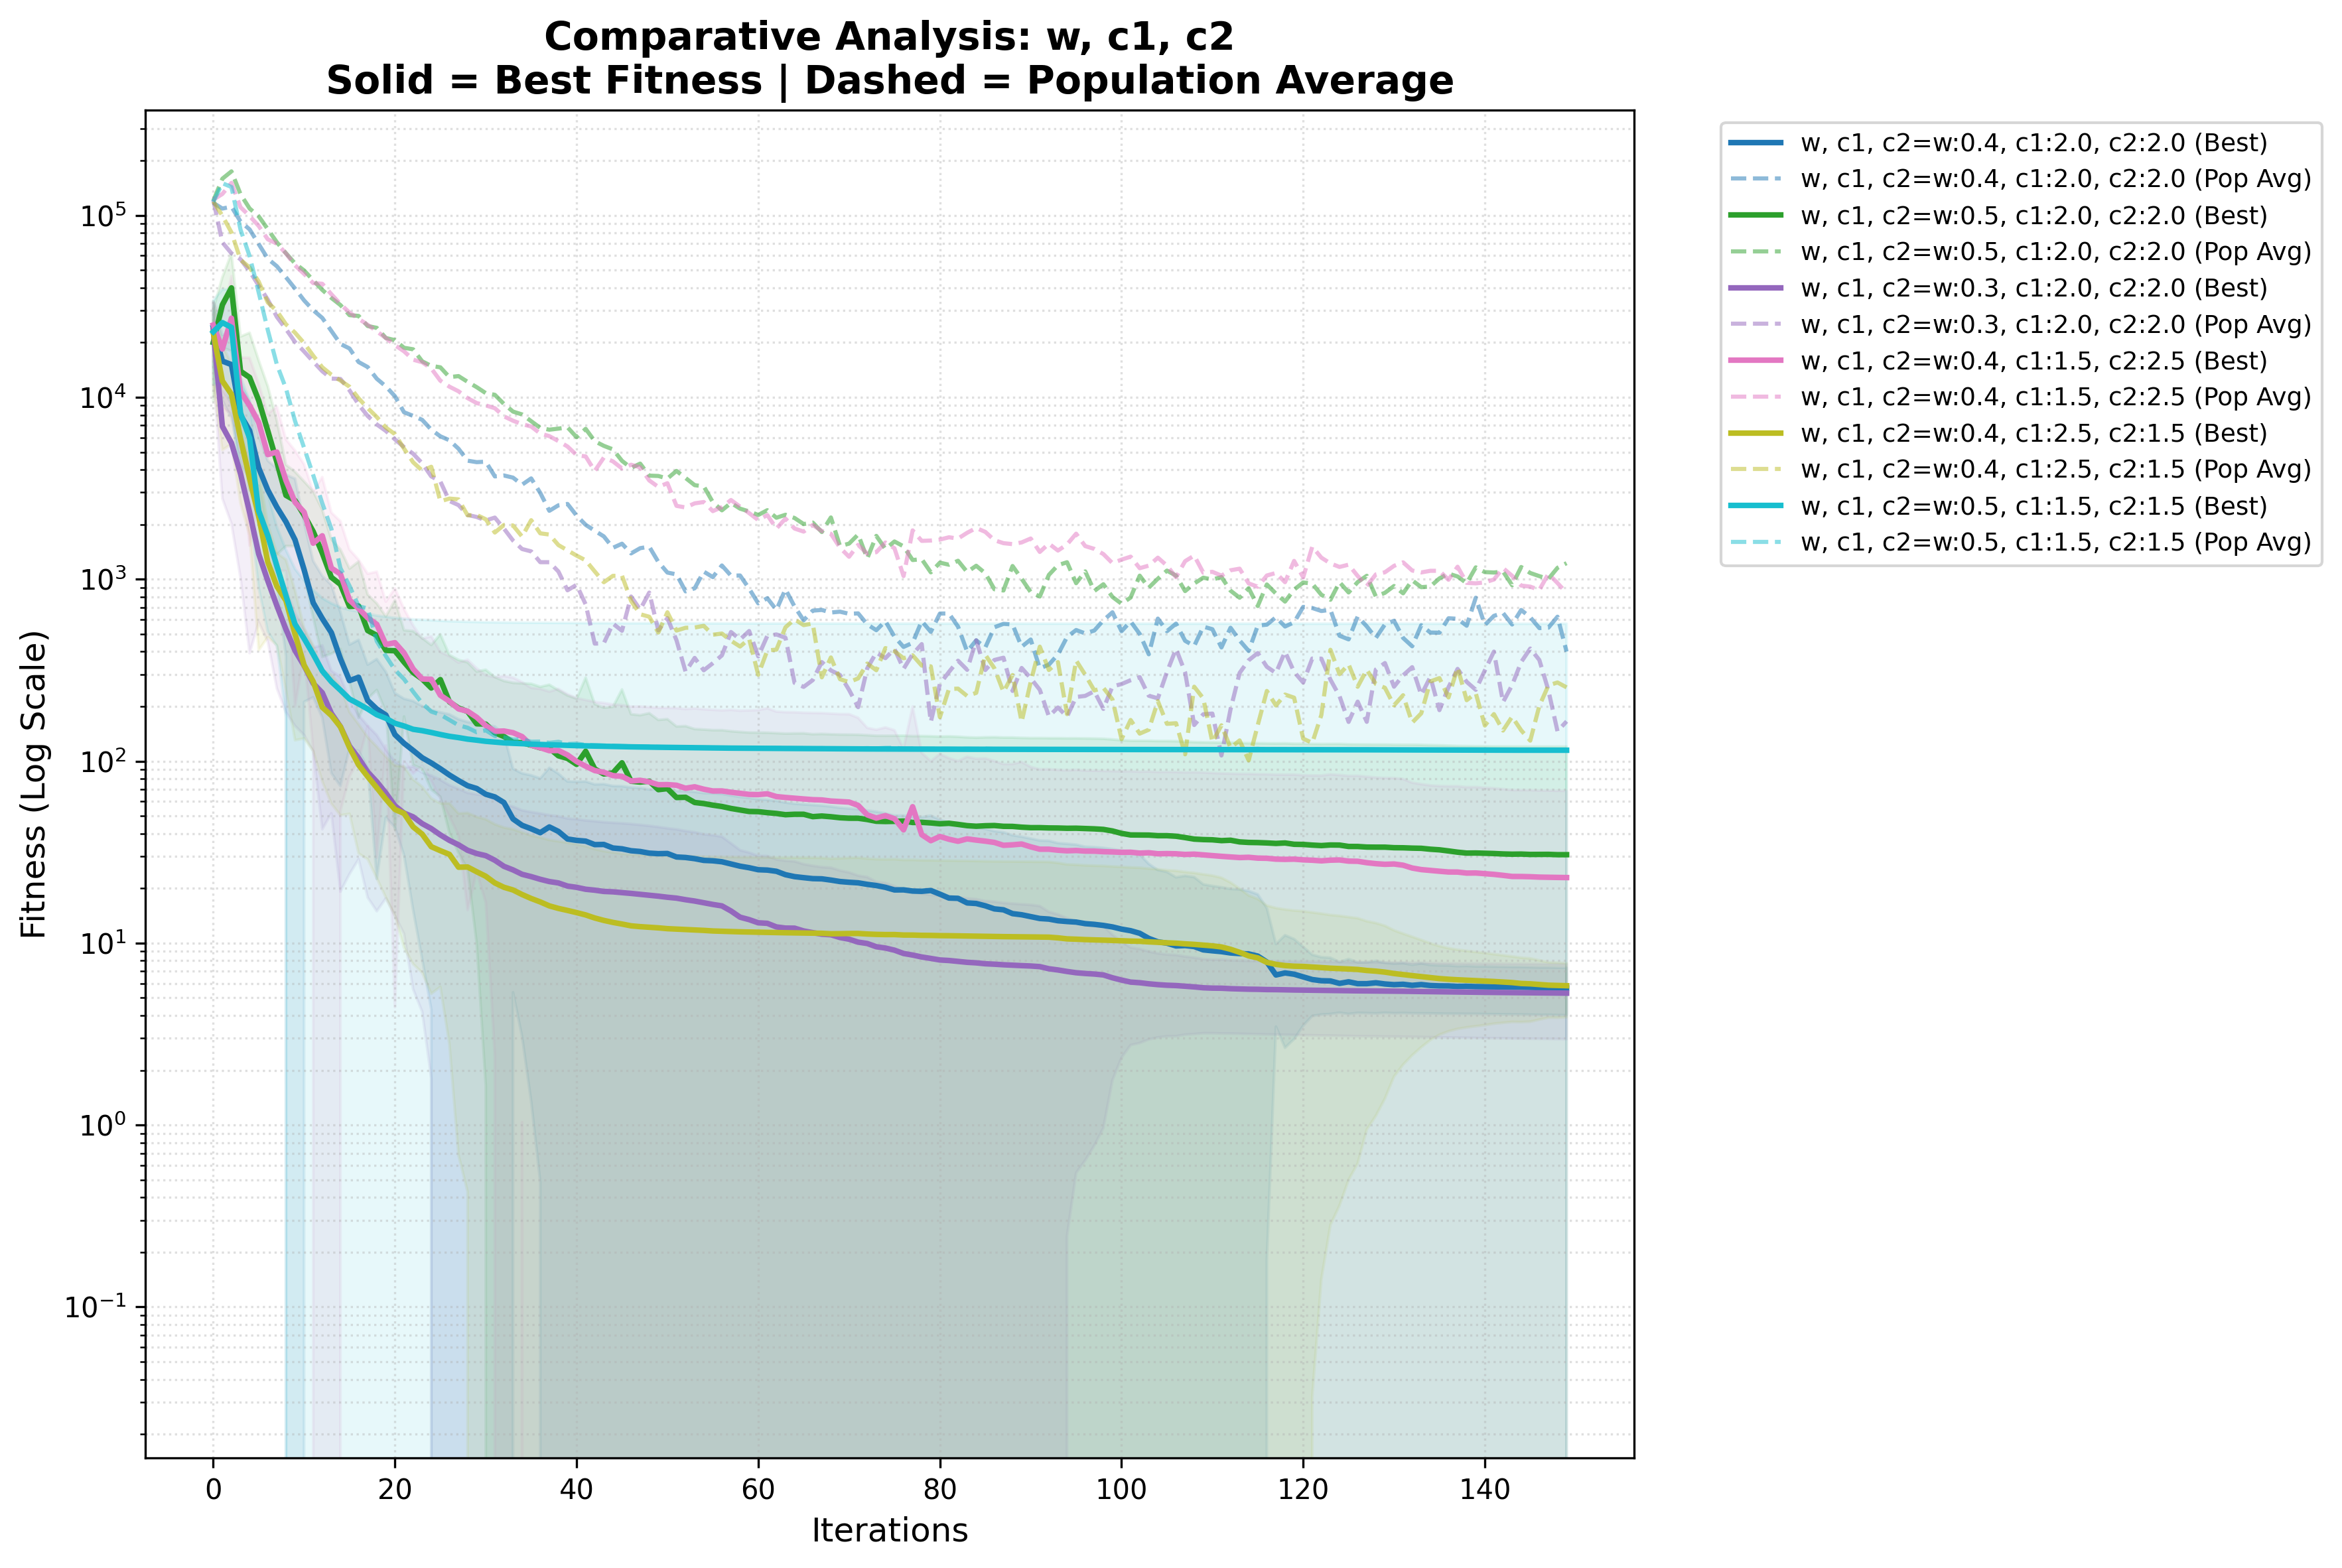
\includegraphics[width=1\linewidth]{comparativa_final_pso_rosenbrock_w_expanded.png}
            \caption{Results of the experiments based on the prior best combination of w, c1 \& c2}
            \label{fig:placeholder}
        \end{figure}

        The better configuration is the one with $w=0.3$, $c_1=2.0$ and $c_2=2.0$, achieving the best average and minimum fitness, but a slighly higher standard deviation. 
        The explanation for this may be in the relation with the inertia weight and the Rosenbrock function, thanks to the steepness of the valley the algorithm may need a lower
         inertia to be able to navigate it, as we can see in the graph, the configuration with $w=0.5$ gets stuck in a local minimum very early, while the one with $w=0.3$ is able to keep improving until the end of the iterations, even if it has a higher standard deviation, which may be explained by the fact that with a lower inertia, particles are more likely to explore different regions of the search space, which can lead to a wider range of fitness values and therefore a higher standard deviation.
            
        \item \textbf{Population}
        
        Just as with the previous section, the greater the quantity of individuals the better were the results, we can see this clearly in the following table:

        \begin{table}[H]
        \centering
        \begin{tabular}{c c c c}
        \hline
        Population & Avg Fit & Min Fit & Std Dev \\
        \hline
        30  & 8.415171 & 0.006544 & 15.978480 \\
        50  & 15.860228 & 0.214079 & 32.603365 \\
        200 & 4.244384  & 0.076317 & 1.583131 \\
        600 & 3.325720  & 0.015000 & 1.765081 \\
        \hline
        \end{tabular}
        \caption{Results PSO – Rosenbrock 10D}
        \end{table}

        After looking at the data, we can clearly see the big impact population has on Rosenbrock, as the average fitness greatly dimishes with high populations. Nontheless, a strange phenomenon happens with the minimum fitness, as the best solution found with a population of 30 is better than the one found with a population of 50, which can be explained by the stochastic nature of the algorithm, as well as the high difficulty of the Rosenbrock function, which can lead to very different results in different runs, even with the same configuration.  
        
        As always, with the following graph we will be able to better understand the behaviour of the algorithm with different population sizes:
        \begin{figure}[H]
            \centering
            
\includegraphics[width=1\linewidth]{comparativa_final_pso_rosenbrock_pop.png}
            \caption{Results of the experiments based on population}
            \label{fig:placeholder}
        \end{figure}
        
        Here the difference between the lowest 2 populations and the highest 2 is even more clear, as with 30 and 50 individuals, the algorithm gets stuck in a local minimum very early, while with 200 and 600 it falls later on, although it looks like it still gets stuck. 
        Basically, with a larger population, the algorithm is able to explore more of the search space and therefore has a higher chance of finding better solutions on Rosenbrock's valley, while with a smaller population, the algorithm may get stuck in local minimums more easily.
        With the average of population average, the worst one is again the one with 600 individuals, just as we saw in the Griewank function, and for the same reasons.

        \item \textbf{Number of Iterations}
        
            The results of the different number of iterations were the following:

        \begin{table}[H]
        \centering
        \begin{tabular}{c c c c}
        \hline
        Iterations & Avg Fit & Min Fit & Std Dev \\
        \hline
        150 & 3.492052 & 0.057507 & 1.208589 \\
        300 & 2.718393 & 0.587443 & 0.740450 \\
        600 & 1.648496 & 0.000239 & 0.834917 \\
        \hline
        \end{tabular}
        \caption{Results PSO – Rosenbrock 10D}
        \end{table}
        We can see that, here as well, there's more impact from this variable than in the Griewank function, as the difficulty of Rosenbrock makes the algorithm need more 
        time to find good solutions. The minimum fitness value for 600 iterations is really small, meaning that the algorithm was able to find a solution very close to the global minimum, which is a great result considering the difficulty of the function. 
        The minimum was even better than the best from Griewank, which is explained by the fact that Rosenbrock is a unimodal function, so once the algorithm finds the valley, it can keep improving until it reaches a very good solution, while in Griewank, the algorithm can get stuck in local minimums and therefore not be able to find such good solutions.
        Another curious thing is that the average fitness for 300 iterations is worse than for 150 iterations, which can also be attributed to stochasticity.
        \begin{figure}[H]
            \centering
            
\includegraphics[width=1\linewidth]{comparativa_final_pso_rosenbrock_iterations.png}
            \caption{Results of the experiments based on iterations}
            \label{fig:placeholder}
        \end{figure}
        The graph presented is really similar to the one from the Griewank function, with no sudden drop of fitness at the end of the iterations, but with a steady improvement over time. 
\end{itemize}    


\subsubsection{Conclusions on PSO}
Along this section, we have been able to see the performance of the PSO algorithm on two different fitness functions, with different natures and difficulties. We have seen how the parameters of the algorithm can greatly impact its performance, and how finding the right balance between exploration and exploitation is crucial for achieving good results.
In the Griewank function, which is a multimodal function with many local minimums, we found that the best configuration was one with low inertia and higher cognitive component, which allowed the particles to explore more independently and avoid getting stuck in local minimums. In the Rosenbrock function, which is a unimodal function with a narrow valley, we found that the best configuration was one with even lower inertia, which allowed the particles to navigate the steep valley more effectively.
In both functions, we also saw that increasing the population size generally led to better performance, as it allowed for a more diverse search of the solution space and reduced the chances of getting stuck in local minimums. Additionally, we observed that increasing the number of iterations can lead to better results, but there may be a point of diminishing returns where additional iterations do not lead to significant improvements in fitness.
Overall, the PSO algorithm showed good performance on both functions, but the choice of parameters was crucial for achieving good results, and the optimal parameters varied depending on the nature of the fitness function being optimized.

\subsection{Differential Evolution }
In this section we will perform the same experiments as with PSO, but with the DE algorithm, testing the same variables in the same order, and of course, with the same fitness functions.

\subsubsection{Griewank function with DE}
\paragraph{Discussion of Results}


    \begin{itemize} 
        \item \textbf{F and CR}
        
            In DE, the variable F is the mutation factor, which controls how much the mutant vector is influenced by the difference between two randomly selected individuals. A higher F encourages more exploration, while a lower F promotes exploitation. The variable CR is the crossover rate, which determines the probability of components being inherited from the mutant vector versus the target vector. A higher CR allows for more mixing of solutions, while a lower CR leads to more conservative updates.


            For these variables we selected the following initial configurations, trying to cover a wide range of values to test different scenarios of exploration and exploitation:
    
                \begin{table}[H]
                    \centering
                    \begin{tabular}{c c c c l}
                    \hline
                    \textbf{Config} & \textbf{F} & \textbf{CR} & \textbf{Description} \\
                    \hline
                    1 & 0.5 & 0.3 & Moderate mutation, low crossover \\
                    2 & 0.7 & 0.5 & Balanced configuration \\
                    3 & 0.5 & 0.9 & Moderate mutation, high crossover \\
                    4 & 0.9 & 0.9 & High exploration (both F and CR high)\\
                    \hline
                    \end{tabular}
                    \caption{Parameter configurations used in the experiments for DE.}
                \end{table}

            Their final results were the following:
                \begin{table}[H]
                    \centering
                    \begin{tabular}{c c c c c}
                    \hline
                    $F$ & CR & Avg Fit & Min Fit & Std Dev \\
                    \hline
                    0.5 & 0.3 & 0.333598 & 0.181127 & 0.073268 \\
                    0.7 & 0.5 & 0.572442 & 0.368196 & 0.097561 \\
                    0.5 & 0.9 & 0.446446 & 0.252065 & 0.106417 \\
                    0.9 & 0.9 & 1.423798 & 1.094365 & 0.168782 \\
                    \hline
                    \end{tabular}
                    \caption{Results DE – Griewank 10D}
                  
                \end{table}
                
                We can observe how the configuration with $F=0.5$ and $CR=0.3$ achieved the best average fitness and minimum fitness, while also maintaining a relatively low standard deviation compared to the other configurations. 
                There's also a clear trend that as we increase F and CR, the performance of the algorithm worsens, which is explained by the fact that with higher values of F and CR, the algorithm becomes more exploratory, which can lead to better solutions in some cases, but it can also lead to worse solutions if the algorithm is not able to effectively exploit the good solutions it finds. In this case, it seems that the higher values of F and CR are leading to worse performance, the algorithm may be struggling to find good solutions in the search space.
                 The configuration with $F=0.9$ and $CR=0.9$ shows a particularly poor performance, which is likely due to the fact that with such high values of F and CR, the algorithm is essentially performing a random search, which is not effective for finding good solutions in a complex search space like Griewank's.
                
                 The comparative graph gives us more information about the behaviour of these configurations during all the iterations:
                \begin{figure}[H]
                    \centering
                    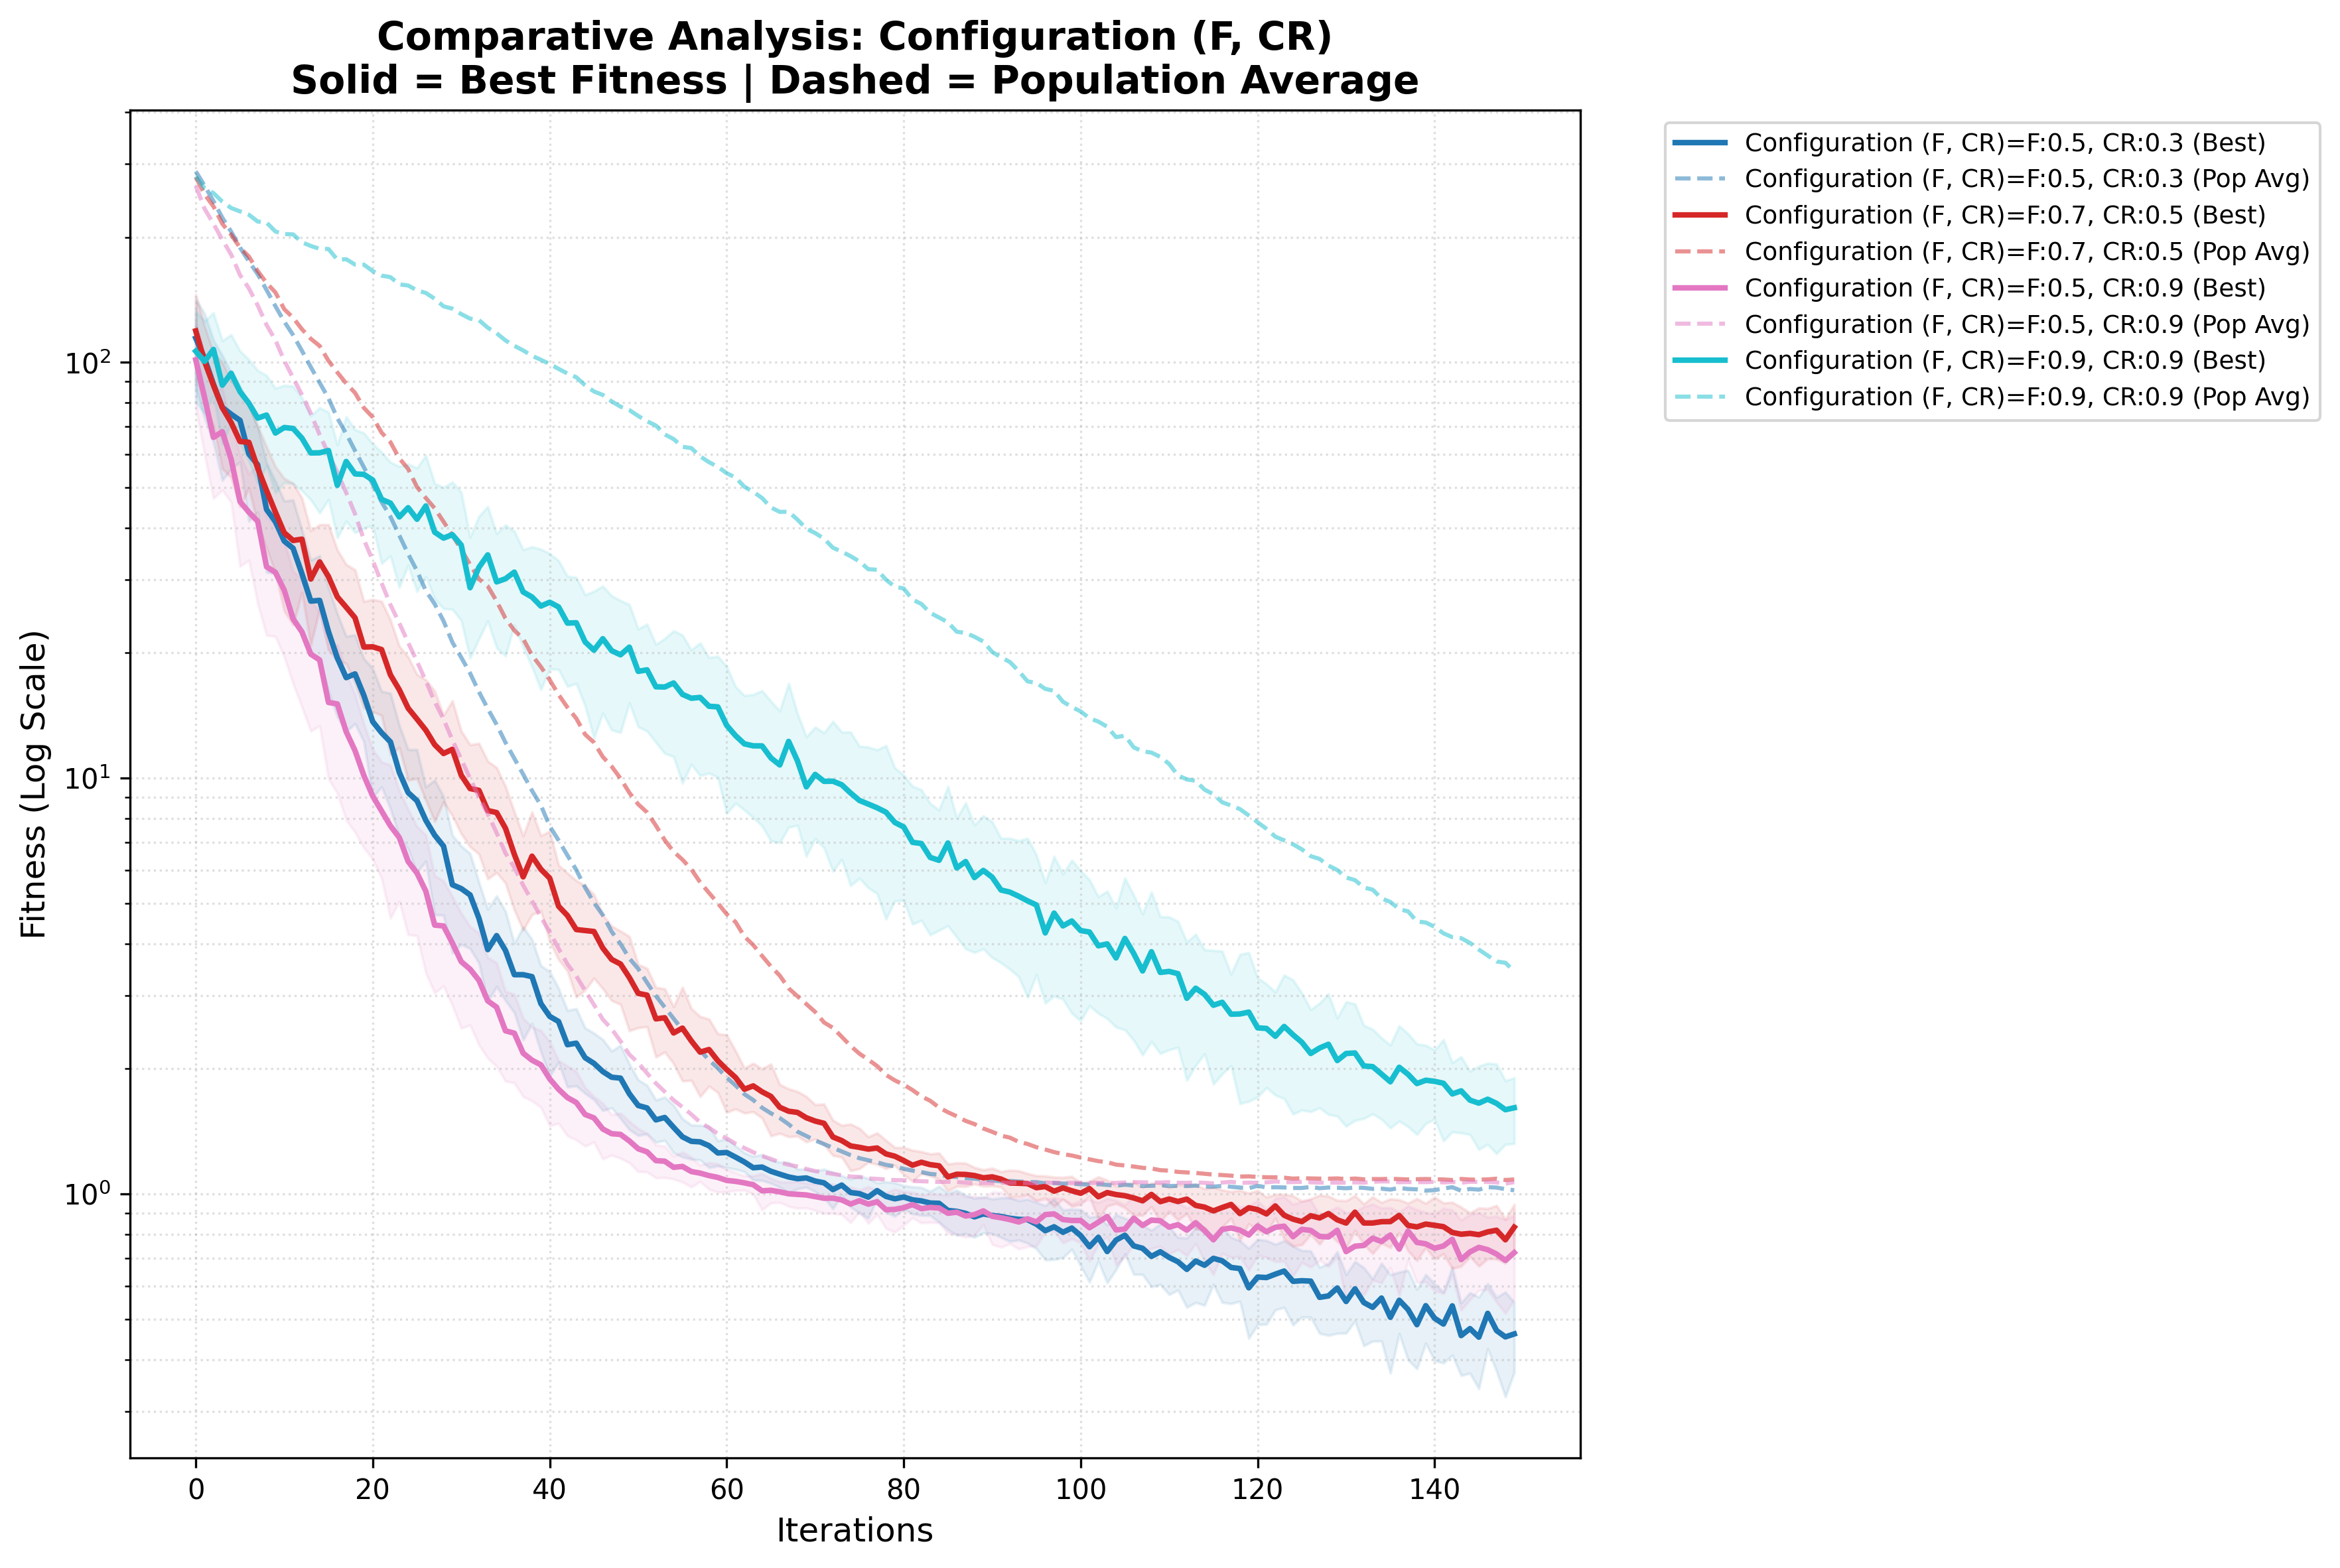
\includegraphics[width=1\linewidth]{comparativa_final_de_griewank_w.png}
                    \caption{Comparison of different F and CR configurations on the Griewank function.}
                    \label{fig:placeholder}
                \end{figure}
                
        By looking at this graph, there's a particularity that keeps our attention, the configuration with $F=0.9$ and $CR=0.9$ keeps consistently above the others but it doesn't seem to have fallen into a local minimum, it keeps improving remarkably,
        whereas the others seem to have a high drop at the beggining and then they improve at a much slower pace. The only one that seems to also keep improving at a good pace is the winner configuration. This makes us question wether with more iterations, the worst configuration could have improved significantly.
        However, this steady improvement is probably driven by its ability to preserve genetic diversity, and explore more extensively the search space, but its large mutation and crossover rates prevent it from fine-tuning solutions within the narrow basin of the global optimum. In contrast, the better-performing configurations benefit from smaller, more precise steps that allow them to exploit promising regions more effectively.    
        
        After some deliberation, we decided to further explore the area around the winning configuration, testing the following values:
         \begin{table}[h!]
                \centering
                \begin{tabular}{c c c c l}
                \hline
                \textbf{Config} & \textbf{F} & \textbf{CR} & \textbf{Description} \\
                \hline
                    1 & 0.5 & 0.3 & Best initial configuration \\
                    2 & 0.6 & 0.3 & Slightly higher F \\
                    3 & 0.6 & 0.4 & Slightly higher F and CR \\
                    4 & 0.5 & 0.5 & Slightly higher CR \\
                    5 & 0.4 & 0.3 & Slightly lower F \\
                    6 & 0.4 & 0.4 & Slightly lower F and higher CR \\
                    7 & 0.3 & 0.3 & Significantly lower F \\
                \hline
                \end{tabular}
                \caption{Additional parameter configurations for fine-tuning around the best initial configuration.}
            \end{table}
        
       
        With their results being the following:
            
          

        \begin{table}[H]
        \centering
            \begin{tabular}{c c c c c}
            \hline
            $F$ & CR & Avg Fit & Min Fit & Std Dev \\
            \hline
            0.5 & 0.3 & 0.304968 & 0.097780 & 0.090108 \\
            0.6 & 0.3 & 0.406095 & 0.190005 & 0.092602 \\
            0.6 & 0.4 & 0.388210 & 0.237818 & 0.089716 \\
            0.5 & 0.5 & 0.373507 & 0.219400 & 0.078861 \\
            0.4 & 0.3 & 0.227031 & 0.084803 & 0.068724 \\
            0.4 & 0.4 & 0.227139 & 0.099584 & 0.061247 \\
            0.3 & 0.3 & 0.116312 & 0.026027 & 0.051400 \\
            \hline
            \end{tabular}

        \caption{Definitive results of F and CR on DE, 10-dimensional Griewank function.}
        \end{table}
        
        Thanks to this exploration, we achieved an even better configuration with $F=0.3$ and $CR=0.3$, which got unbeatable results. This finding is consistent with the previous results, as it further confirms that lower values of F and CR are more effective for this problem, as they allow the algorithm to exploit promising regions better while still maintaining some level of exploration.

        In the following graph we are able to appreciate better the behaviour of these configurations:
        \begin{figure}[H]
            \centering
            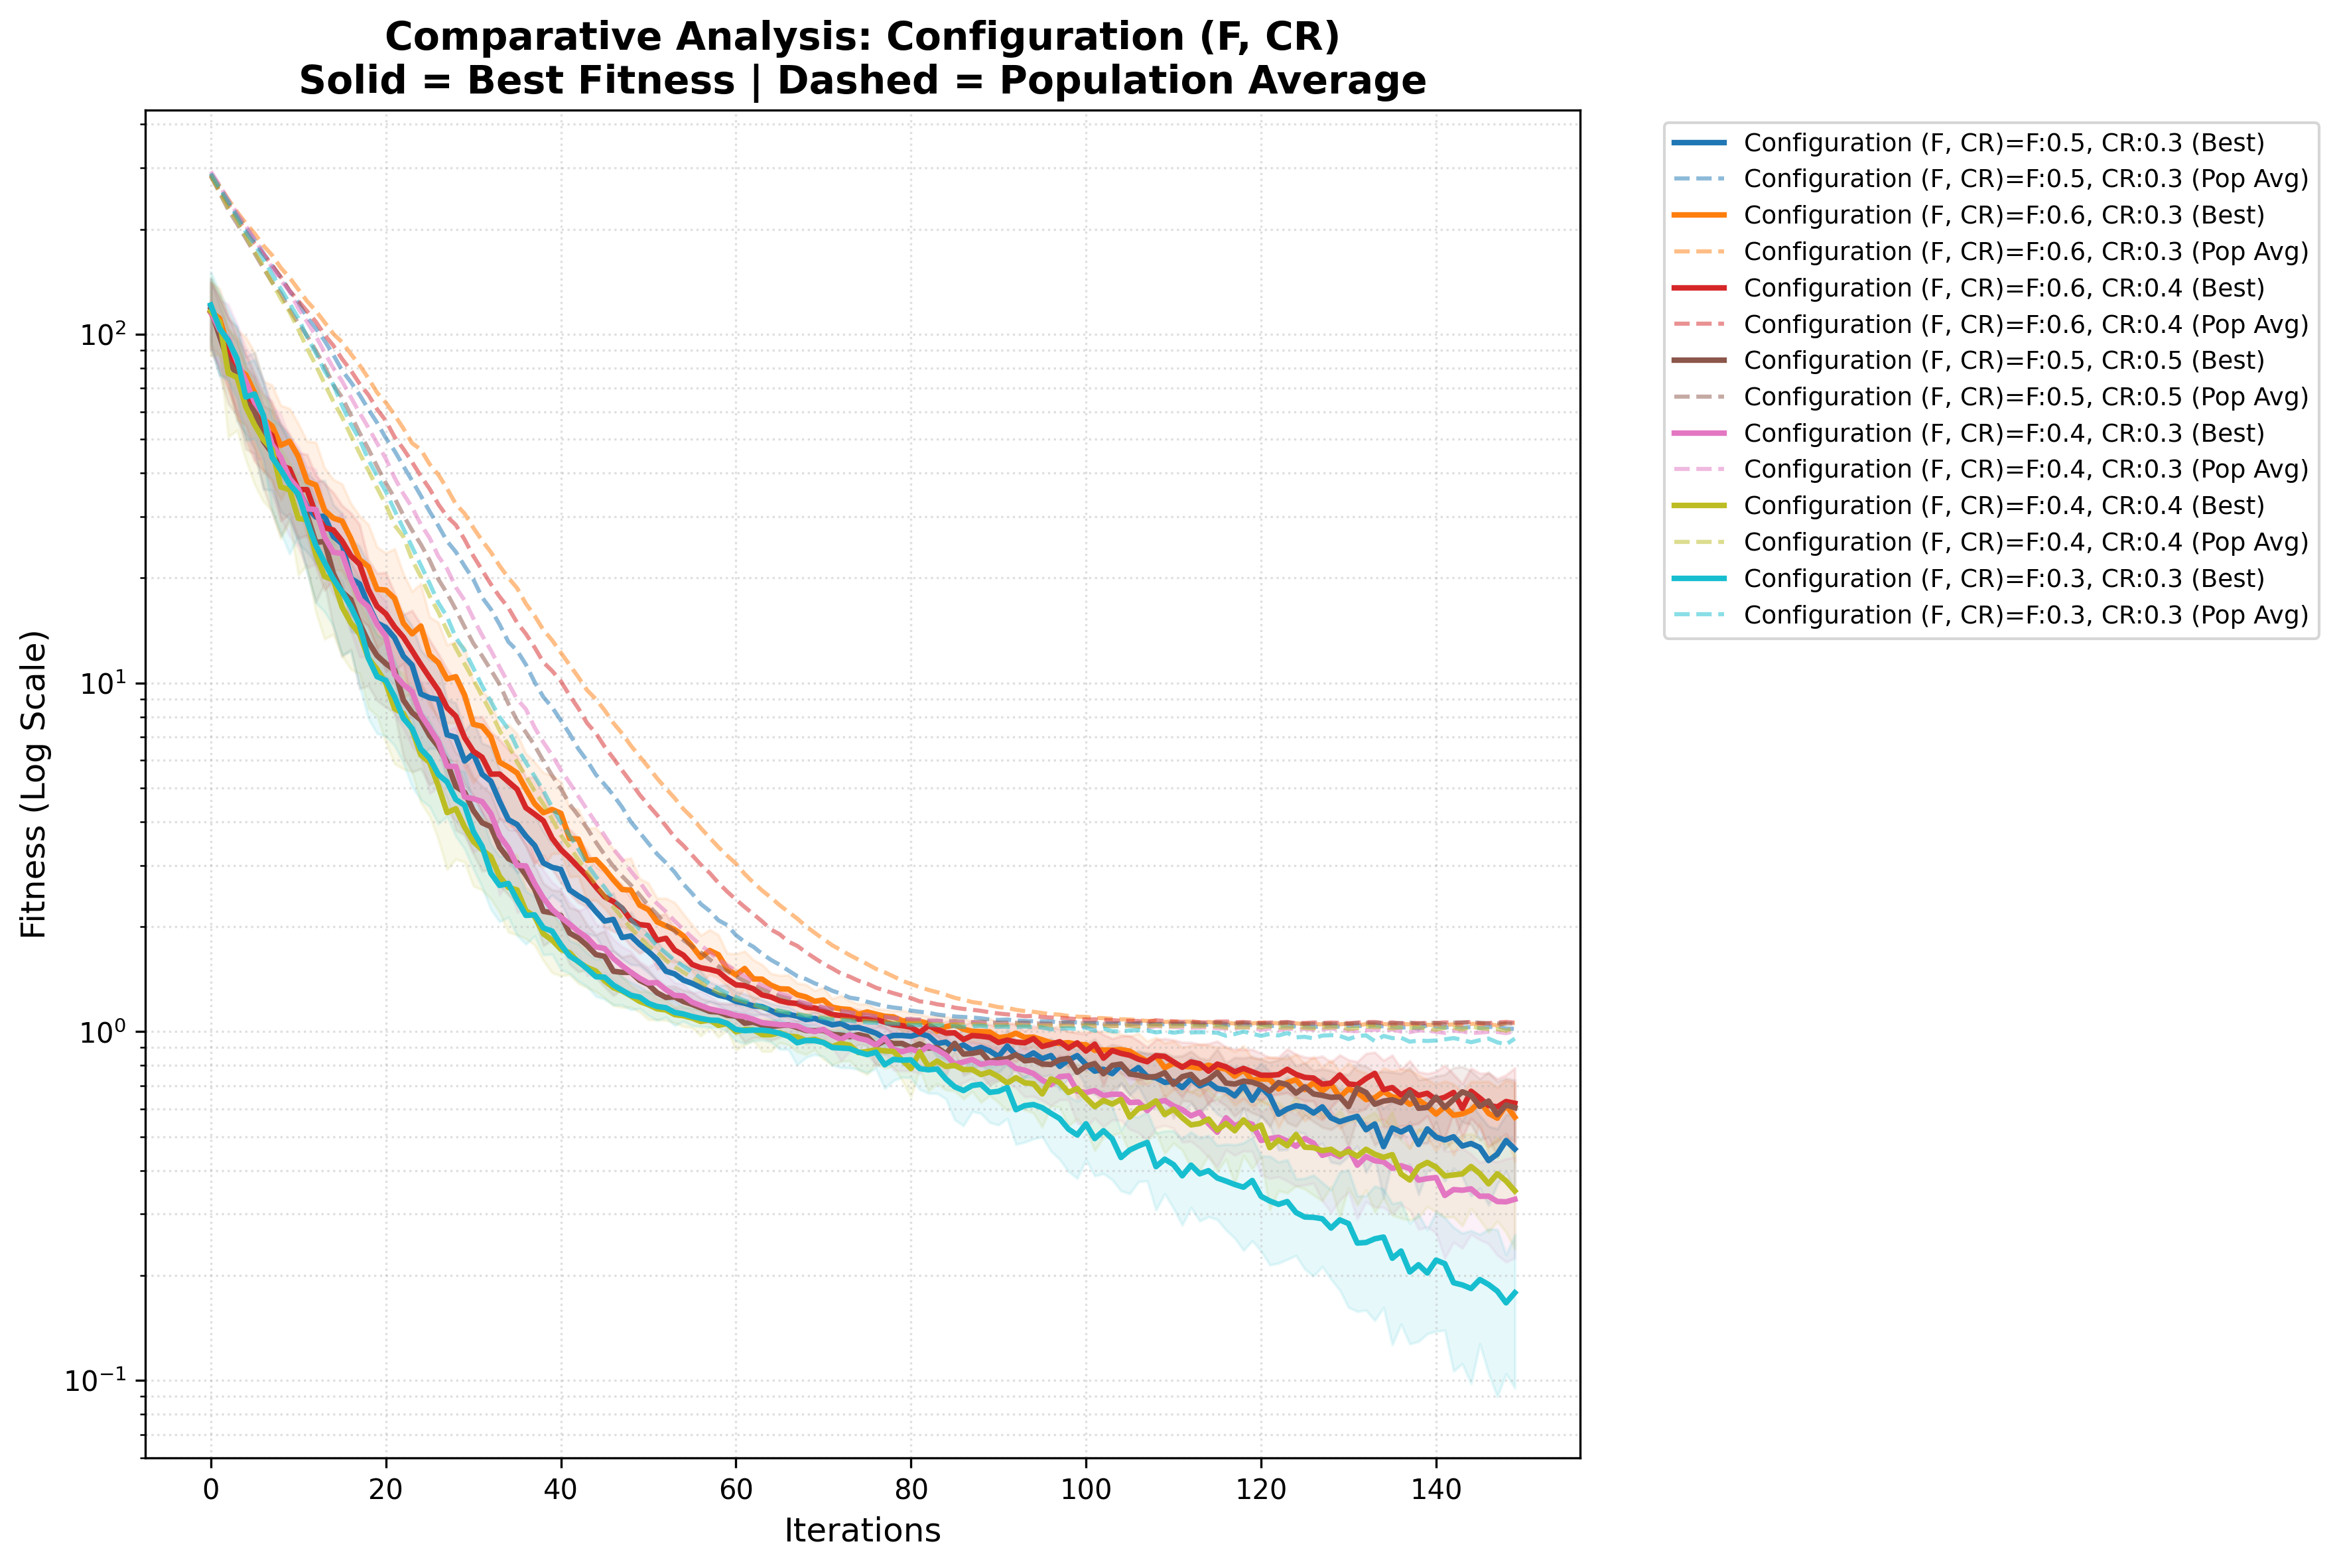
\includegraphics[width=1\linewidth]{comparativa_final_de_griewank_w_expanded.png}
            \caption{Comparison of the best configuration with other similar configurations.}
            \label{fig:placeholder}
        \end{figure}

        There's a clear trend that all the configurations end up with really similar values for their average of population average, not improving soince iteration 80, this is probably due to the sheer quantity of holes (local minimums) in the Griewank function, which makes it so a big number of individuals get stuck in those minimums.
        On the other hand, the minimum fitness keep improving slowly for the majority of the configurations, meaning that some individuals are being able to escape from those minimums.
        The best configuration (light blue) is the one that falls the most at the end of iterations.
        \item \textbf{Population}
        
        Next, we tested the impact of the population size, same values as before, and the results were the following:
        \begin{table}[H]
        \centering
        \begin{tabular}{c c c c}
        \hline
        Population & Avg Fit & Min Fit & Std Dev \\
        \hline
        30  & 0.142707 & 0.043529 & 0.060412 \\
        50  & 0.123638 & 0.024928 & 0.048246 \\
        200 & 0.103649 & 0.056918 & 0.020722 \\
        600 & 0.082491 & 0.037309 & 0.019313 \\
        \hline
        \end{tabular}
        \caption{Results DE – Griewank 10D}
        \end{table}
        It's apparent that increasing the population leads to better average results, because with more individuals there will be more of them that can effectively leave the local minimums.

        In the following graph we can see the behaviour of the algorithm with different population sizes:
        \begin{figure}[H]
            \centering
            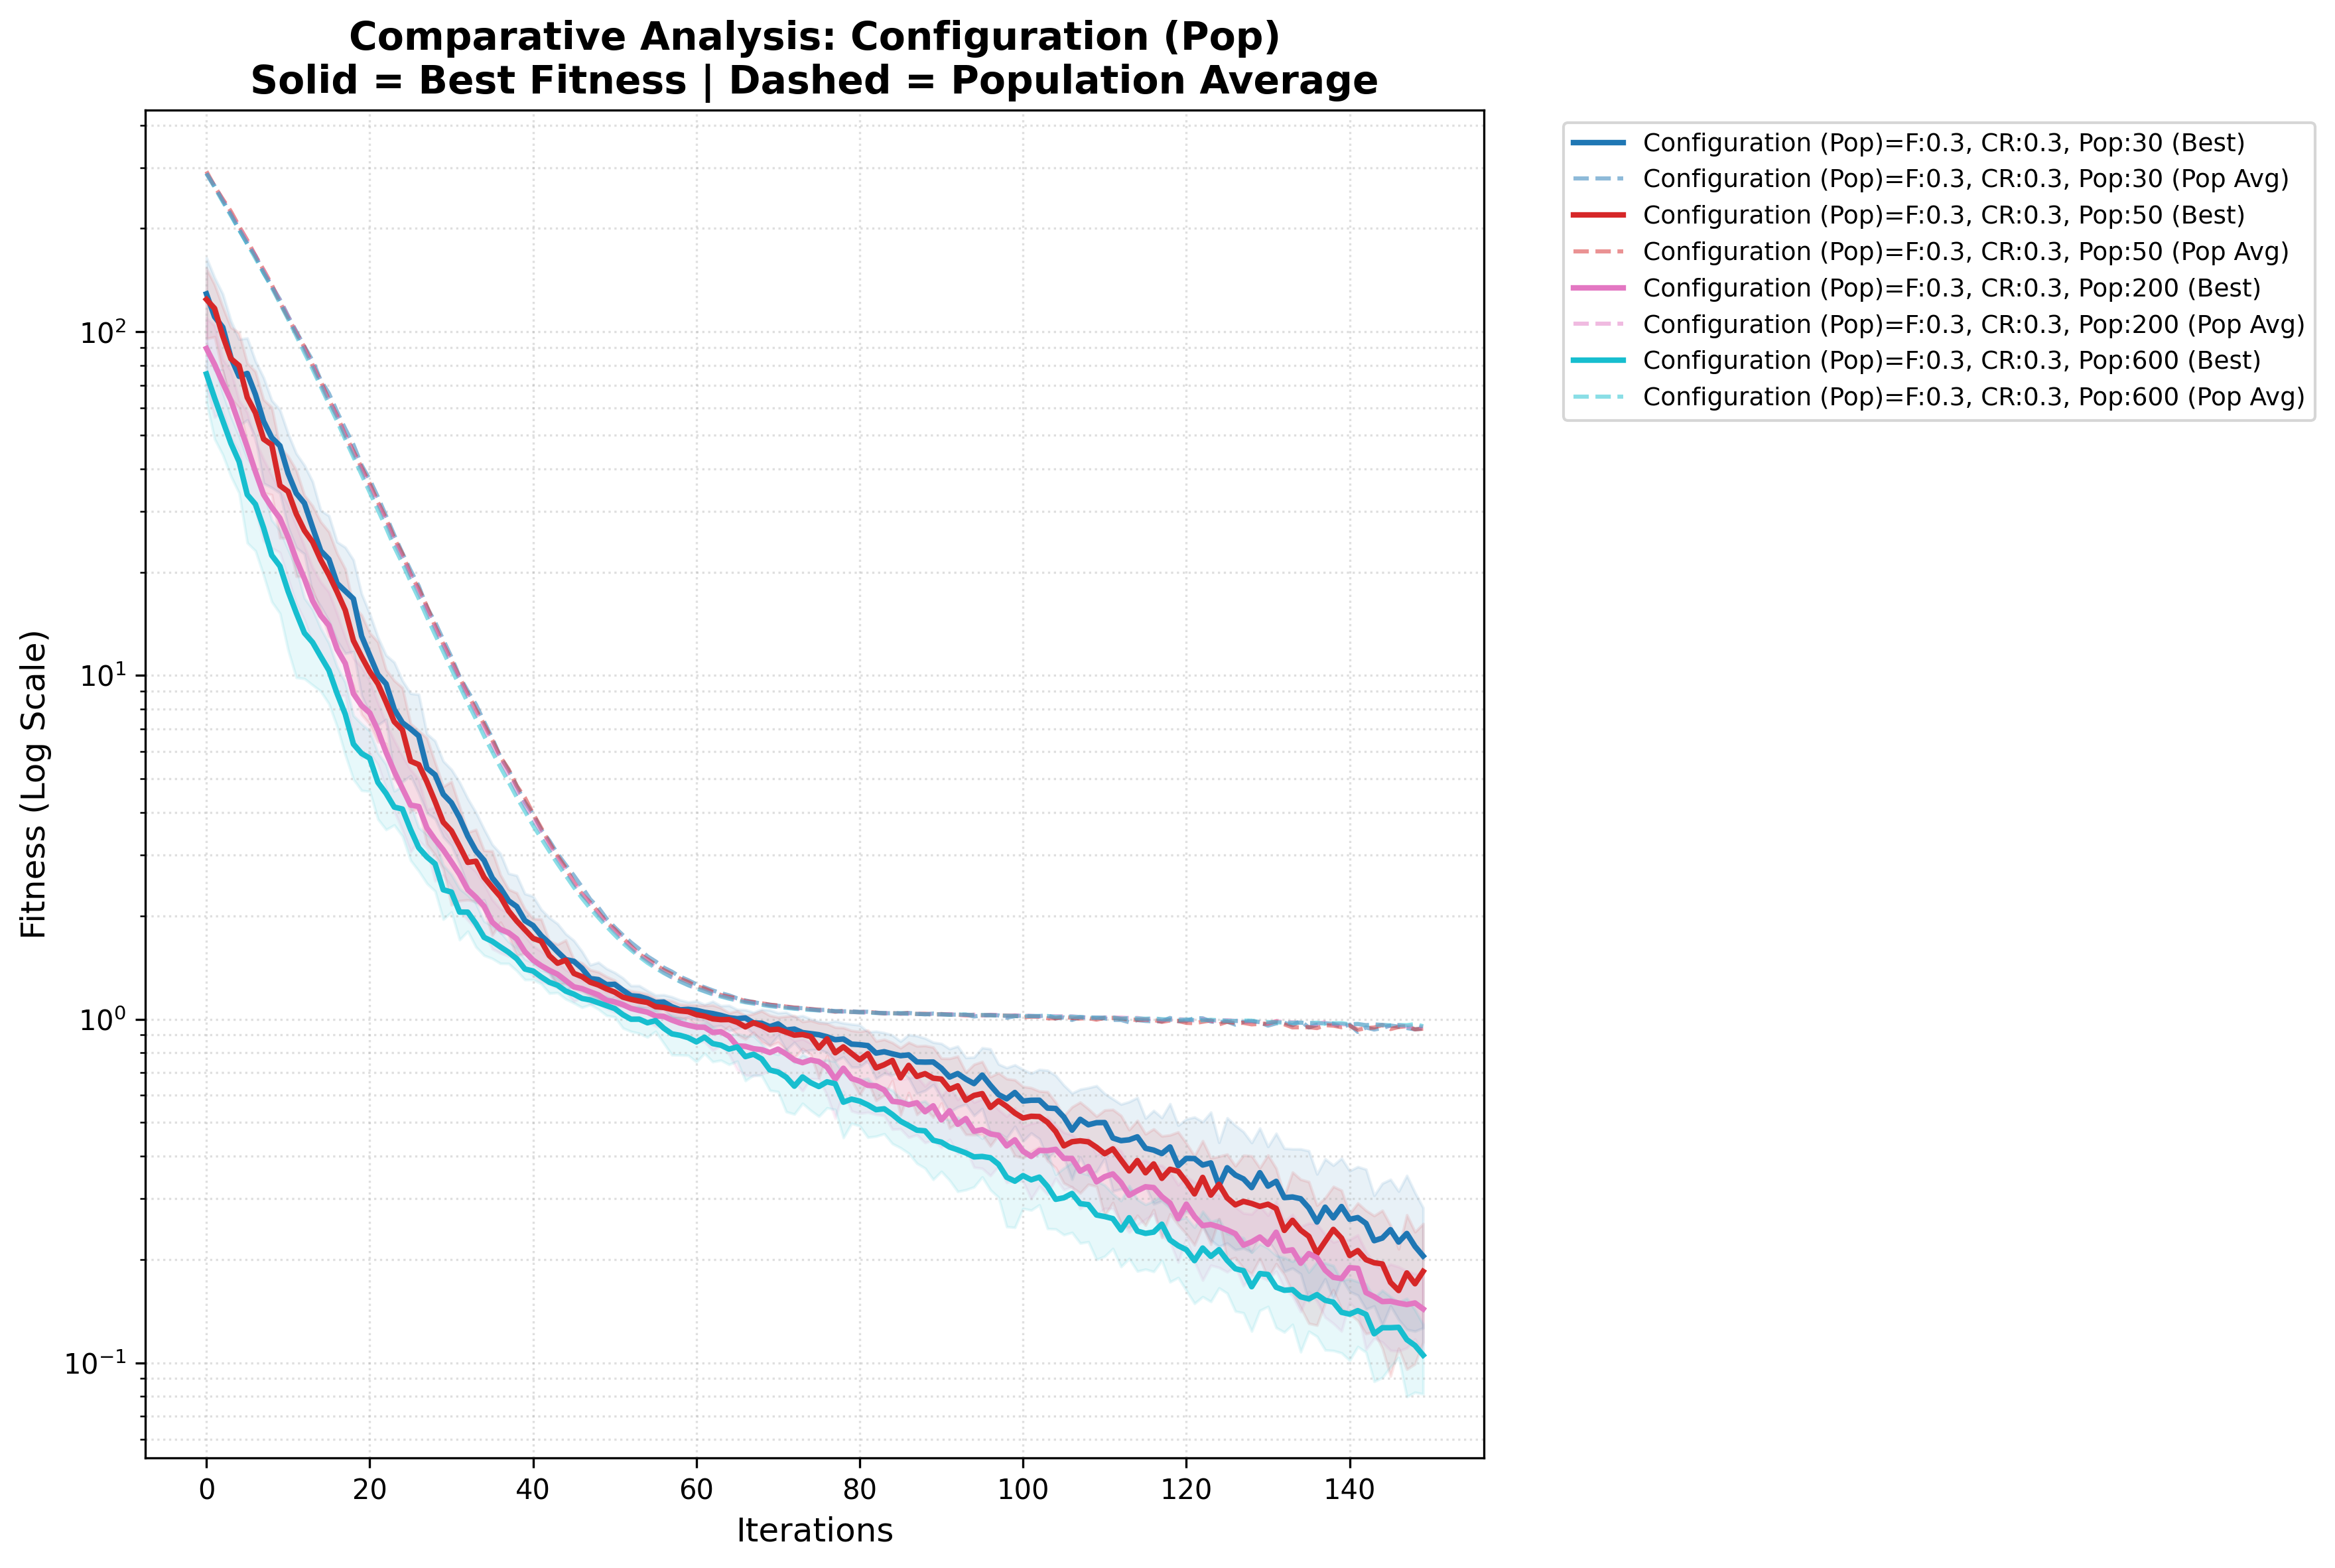
\includegraphics[width=1\linewidth]{comparativa_final_de_griewank_pop.png}
            \caption{Results of the experiments based on population}
            \label{fig:placeholder}
        \end{figure}
       
        We can actually see how, as expected, the algorithm with 600 individuals is consistently better than the rest even though they follow a similar trend.

        \item \textbf{Number of Iterations}
        \item 
        Finally, we tested the impact of the number of iterations, and the results were the following:
        \begin{table}[H]
        \centering
        \begin{tabular}{c c c c}
        \hline
        Iterations & Avg Fit & Min Fit & Std Dev \\
        \hline
        150 & 0.085466 & 0.030789 & 0.017404 \\
        300 & 0.000858 & 0.000097 & 0.000490 \\
        600 & 3.700743e-18 & 0.000000 & 1.992911e-17 \\
        \hline
        \end{tabular}
        \caption{Results DE – Griewank 10D}
        \end{table}
        From past experience, we knew that the bigger the number of iterations, the better the results, but the interesting part
        here was that the sheer amount of improvement made it so the algorithm was able to achieve a perfect result with 600 iterations and a 
        near perfect result with 300 iterations. This shows how powerful DE can be when leaving it enough time to find good solutions.
        
        This behaviour was clearly represented on the following graph:
        \begin{figure}[H]
            \centering
            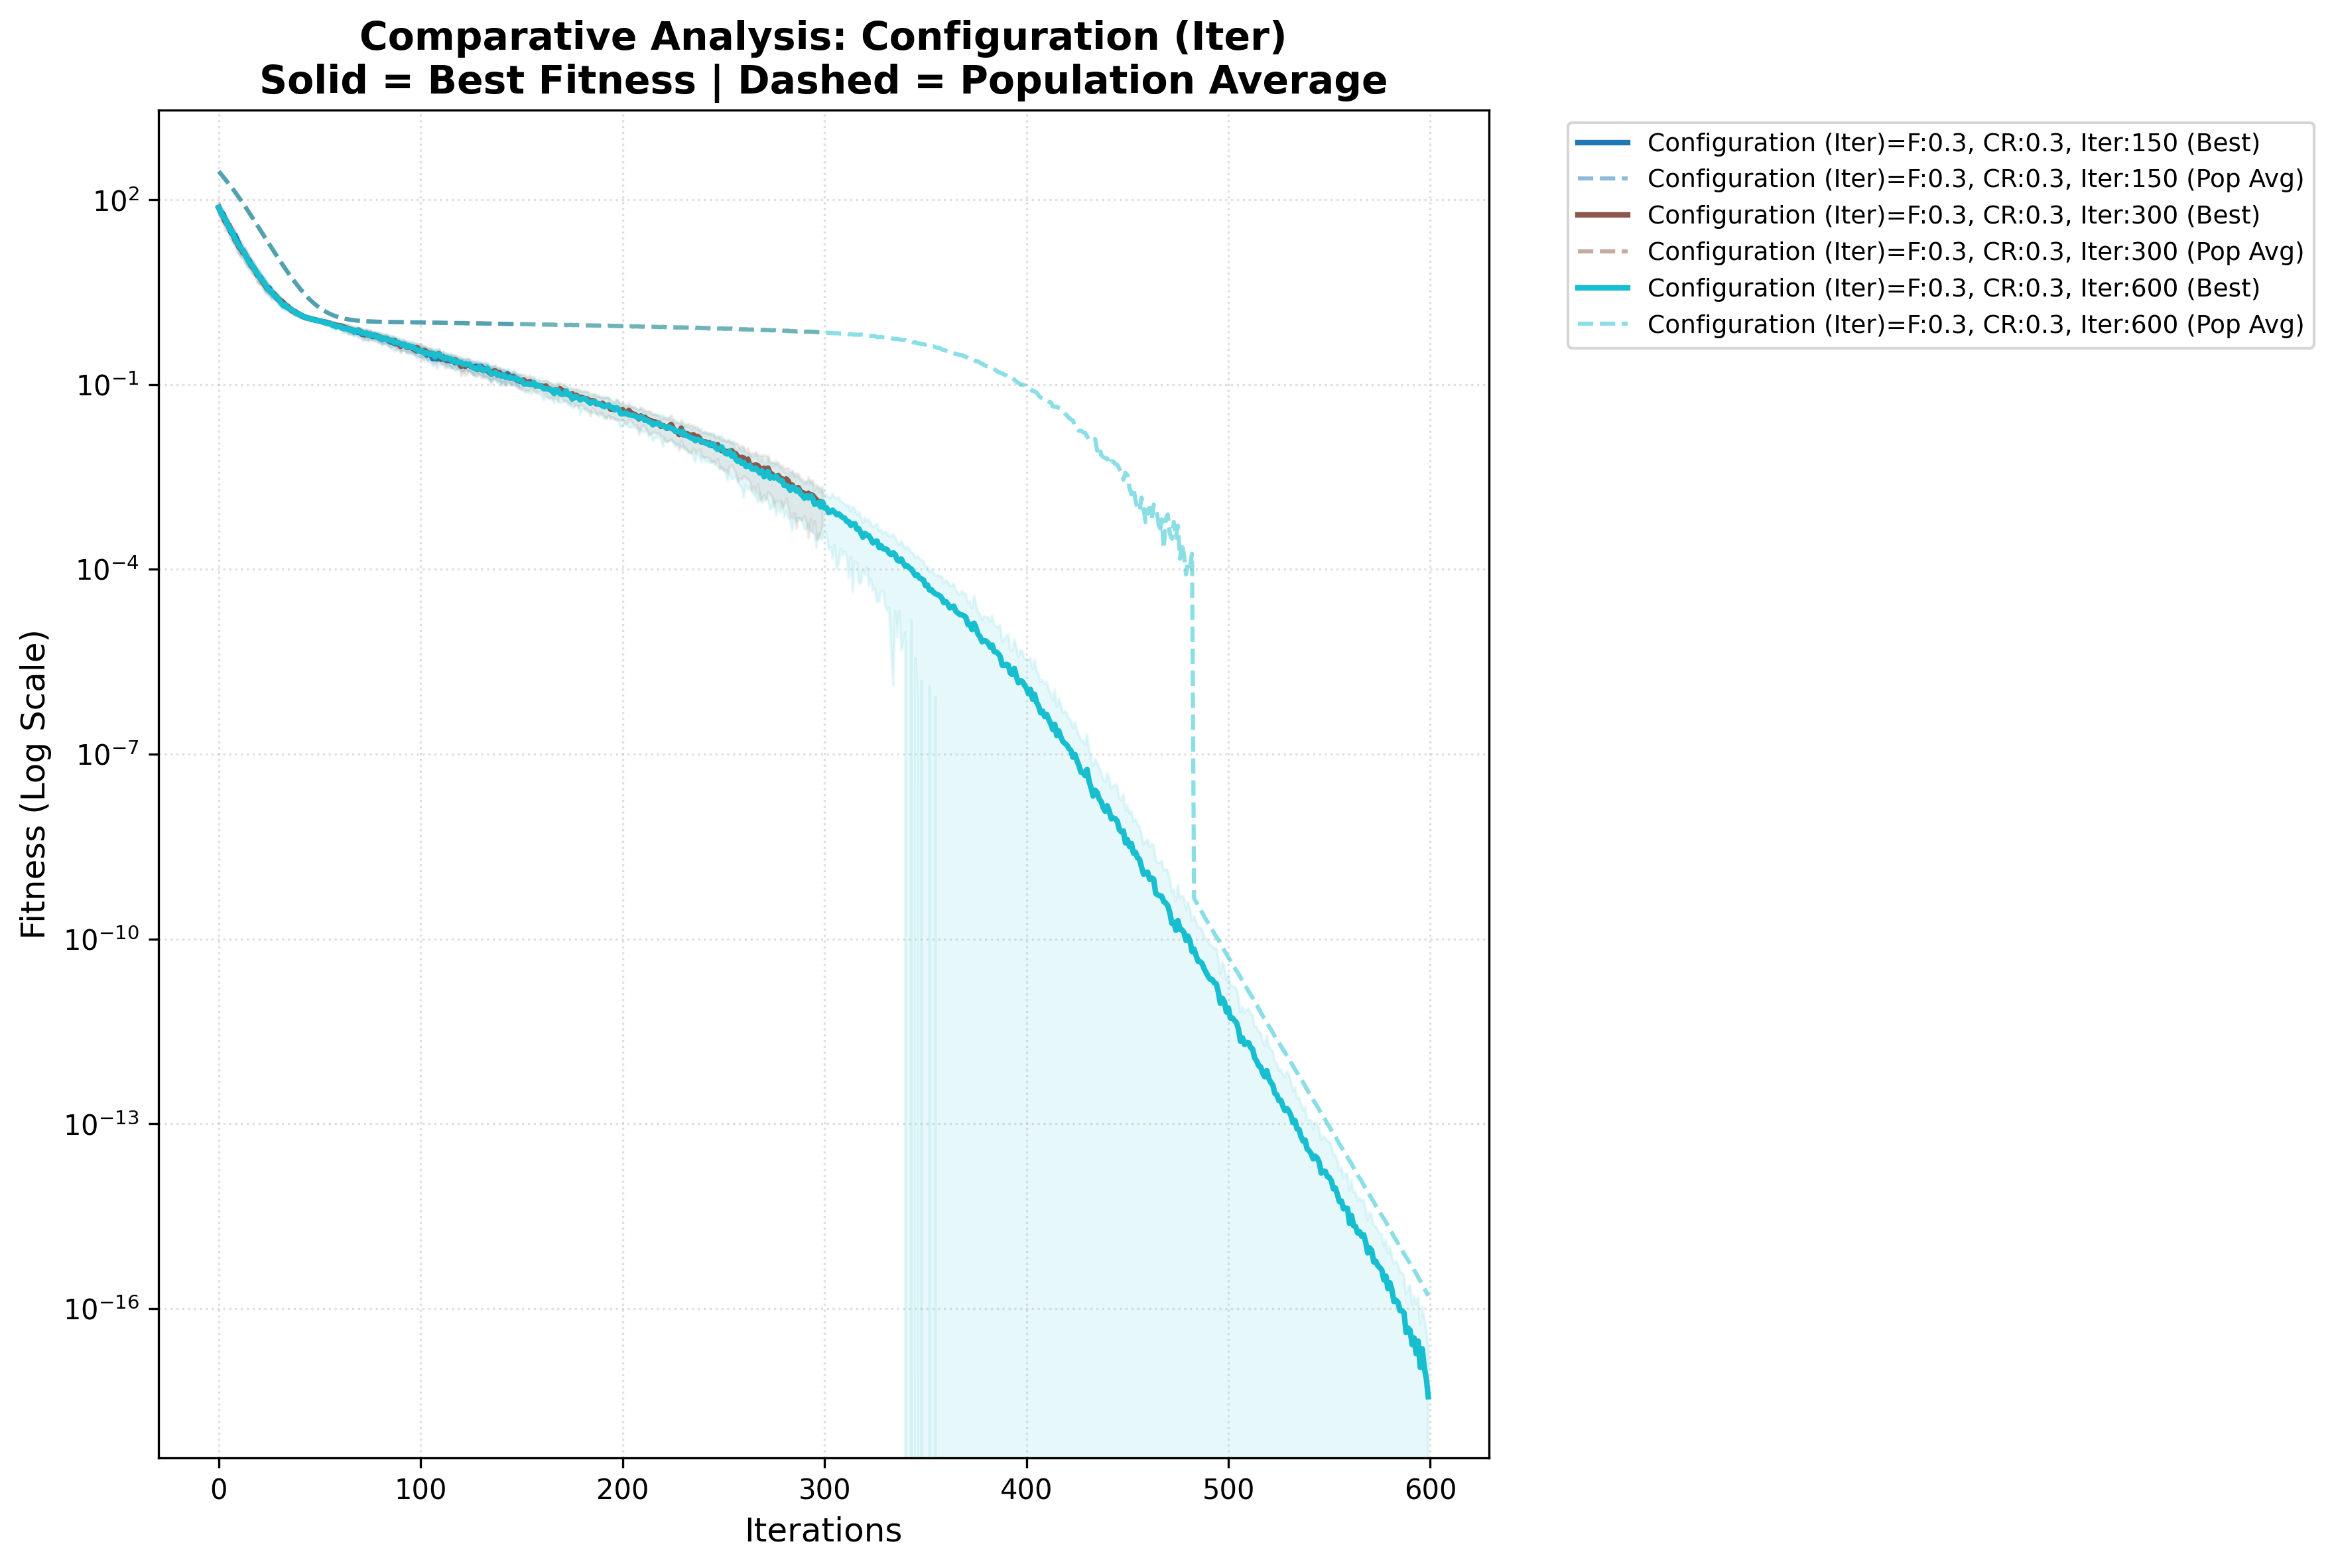
\includegraphics[width=1\linewidth]{comparativa_final_de_griewank_iter.png}
            \caption{Results of the experiments based on iterations}
            \label{fig:placeholder}
        \end{figure}
        As a contrast to the PSO algorithm, in DE we can see a significant drop of fitness within the last 300 iterations. This shows us how
         DE is able to escape from local minimums more effectively than PSO, and therefore iterations have a bigger impact on the results.
        This is consistent with the fact that DE is a more exploratory algorithm than PSO. Also, the average of population average's sudden drop
        before 500 iterations shows the moment when the majority of the individuals in the population were able to escape from local minimums.
    \end{itemize}    
        
\subsubsection{Rosenbrock function with DE}


\paragraph{Discussion of Results}
\begin{itemize} 
        \item \textbf{F and CR}
        
        For the Rosenbrock function, we used the same initial configurations as with the Griewank function, and the results were the following:
        \begin{table}[H]
        \centering
        \begin{tabular}{c c c c c c}
        \hline
        $F$ & $CR$ & Avg Fit & Min Fit & Std Dev \\
        \hline
        0.5 & 0.3 & 10.651966 & 7.185805 & 3.266044 \\
        0.7 & 0.5 & 10.351983 & 7.809374 & 1.921897 \\
        0.5 & 0.9 & 5.532096 & 2.730945 & 1.210683 \\
        0.9 & 0.9 & 28.531120 & 14.829063 & 10.098321 \\
        \hline
        \end{tabular}
        \caption{Results DE – Rosenbrock 10D}
        \end{table}

        Based on these results there's a clear winner, even doubling the average fitness of the second best configuration, which is the one with $F=0.5$ and $CR=0.9$.
        It is clear that, compared to Griewank, in Rosenbrock we need a higher CR, this is probably due to the interdependency of the variables in Rosenbrock, where we need coordinated changes in multiple dimensions to effectively navigate the narrow valley.
        Additionally, it was also expected that the lowest F would give the best performance, as if the mutation factor is too high, the algorithm may not adapt well to the valley, overshooting good solutions.
            The worst configuration is the one with $F=0.9$ and $CR=0.9$, which is consistent with the results from Griewank, as it seems that such high values of F and CR lead to a very exploratory behavior that is not effective for finding good solutions in a complex search space like Rosenbrock's.
            
            The comparative graph gives us more information about the behaviour of these configurations during all the iterations:
        \begin{figure}[H]
            \centering
            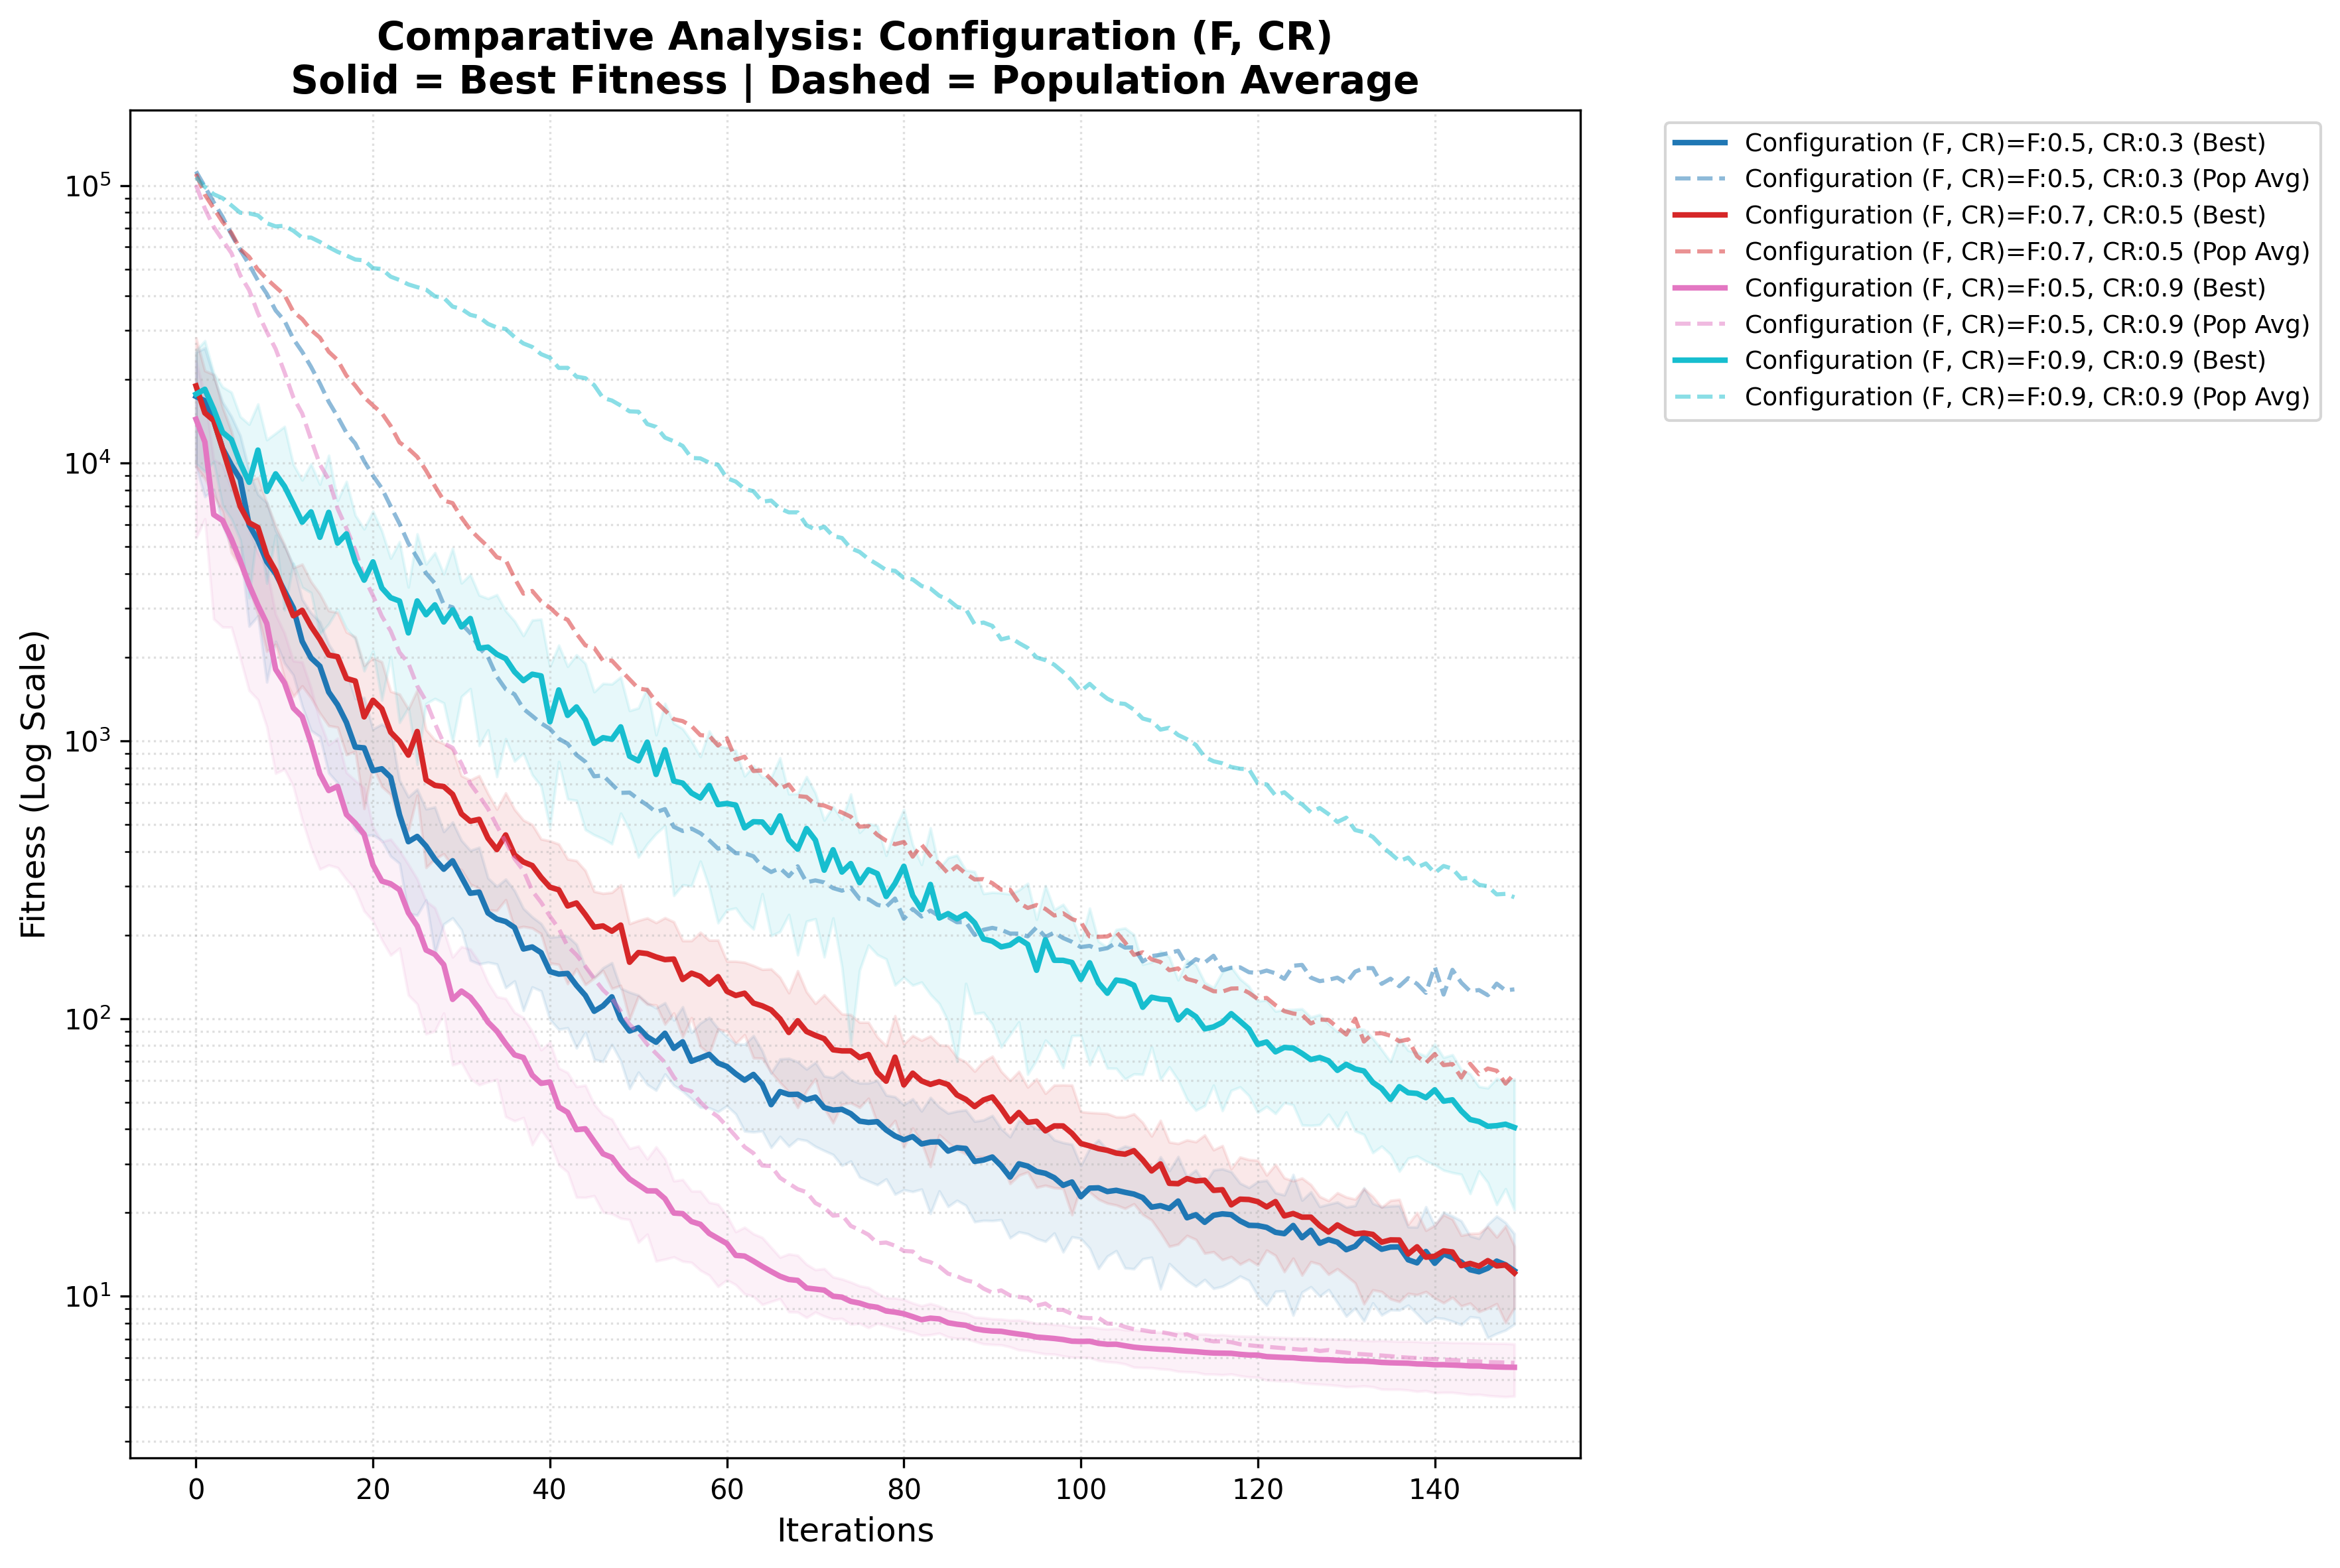
\includegraphics[width=1\linewidth]{comparativa_f_cr_de_rosenbrock.png}
            \caption{Comparison of different F and CR configurations on the Rosenbrock function.}
            \label{fig:placeholder}
        \end{figure}
        
        Our best configuration was the fastest to drop its fitness, but it slowed its pace at around iteration 60, which is probably due to the fact that it got stuck in a local minimum, and
        it wasn't able to escape from it, on the other hand the other configurations seemed to have a more lineal improvement, but were always worse than the best one and even showed
        some slowing down at the end of the iterations.
        It is interesting how the average of the population average for the best configuration converged to its minimum fitness when the minimum was found, this means that
        the majority of the individuals in the population were able to find that good solution. 

            Based on these findings, we decided to further explore the area around the winning configuration, testing the following values:
        
         \begin{table}[H]
                \centering
                \begin{tabular}{c c c c l}
                \hline
                \textbf{Config} & \textbf{F} & \textbf{CR} &  & \textbf{Description} \\
                \hline
                1 & 0.5 & 0.9 & & Best initial configuration \\
                2 & 0.6 & 0.9 & & Slightly higher F \\
                3 & 0.4 & 0.9 & & Slightly lower F \\
                4 & 0.3 & 0.8 & & Slightly lower F and CR \\
                5 & 0.3 & 0.9 & & Lower F and same CR \\
                6 & 0.5 & 0.8 & & Same F and slightly lower CR \\
                \hline
                \end{tabular}
                \caption{Additional parameter configurations for fine-tuning around the best initial configuration.}
        \end{table}
        
        And the results were the following:
        \begin{table}[H]
        \centering
        \begin{tabular}{c c c c c c}
        \hline
        \textbf{F} & \textbf{CR} & \textbf{Avg Fit} & \textbf{Min Fit} & \textbf{Std Dev} \\
        \hline
                  0.5 &            0.9 & 5.880140 & 3.921010 & 0.904368 \\
         0.6 &             0.9 & 6.417211 & 4.913347 & 0.840290 \\
            0.4 &             0.9 & 6.423973 & 3.878515 & 1.026326 \\
            0.3 &             0.8 & 6.675486 & 4.191744 & 1.204428 \\
            0.3 &             0.9 & 7.515228 & 4.510242 & 1.415243 \\
            0.5 &             0.8 & 6.254889 & 4.951439 & 0.770662 \\
        \hline
        \end{tabular}
        \caption{Definitive results of F and CR on DE, 10-dimensional Rosenbrock function.}
        \end{table}
        It seems that the best configuration is still the one with $F=0.5$ and $CR=0.9$, this can mean that the moderate value of F hits the right spot for Rosenbrock, because lower and higher values degraded performance.
        Moreover, it is also consistent that the higher CR is needed for this function, because with F fixed at 0.5, the configuration with CR of 0.8 is worse than the one with CR of 0.9, and with F fixed at 0.3, the configuration with CR of 0.9 is better than the one with CR of 0.8.

        In the following graph we can observe better the permormance of these configurations:
        \begin{figure}[H]
            \centering
            
\includegraphics[width=1\linewidth]{comparativa_f_cr_final_de_rosenbrock.png}
            \caption{Results of the experiments based on the prior best combination of F \& CR}
            \label{fig:placeholder}
        \end{figure}

        We can see how they are all really similar, but there's a trend in a sense that those with the lowest values of F tend to converge faster,
        it makes sense considereing that the lower the value the more fine tuning the algorithm is able to do. Nonetheless,
        at the end of iterations we can appreciate how the configurations with higher F are able to catch up and even surpass them, as it happens with the best configuration.
        \item \textbf{Population}
        
        The results of the different population sizes were the following:
        

        \begin{table}[H]
        \centering
        \begin{tabular}{c c c c}
        \hline
        Population & Avg Fit & Min Fit & Std Dev \\
        \hline
        30  & 6.926613 & 3.974404 & 1.135637 \\
        50  & 6.370480 & 5.257854 & 0.710968 \\
        200 & 5.775775 & 5.141781 & 0.213696 \\
        600 & 5.644490 & 4.981572 & 0.242364 \\
        \hline
        \end{tabular}
        \caption{Results DE – Rosenbrock 10D}
        \end{table}

        In this case, the impact of population enlargement is not as significant as in the Griewank function, 
        but, as always, it still shows that with more individuals the algorithm is able to find better solutions.
        
        The following graph gives us a better understanding of the behaviour of the algorithm with different population sizes:
        \begin{figure}[H]
            \centering
            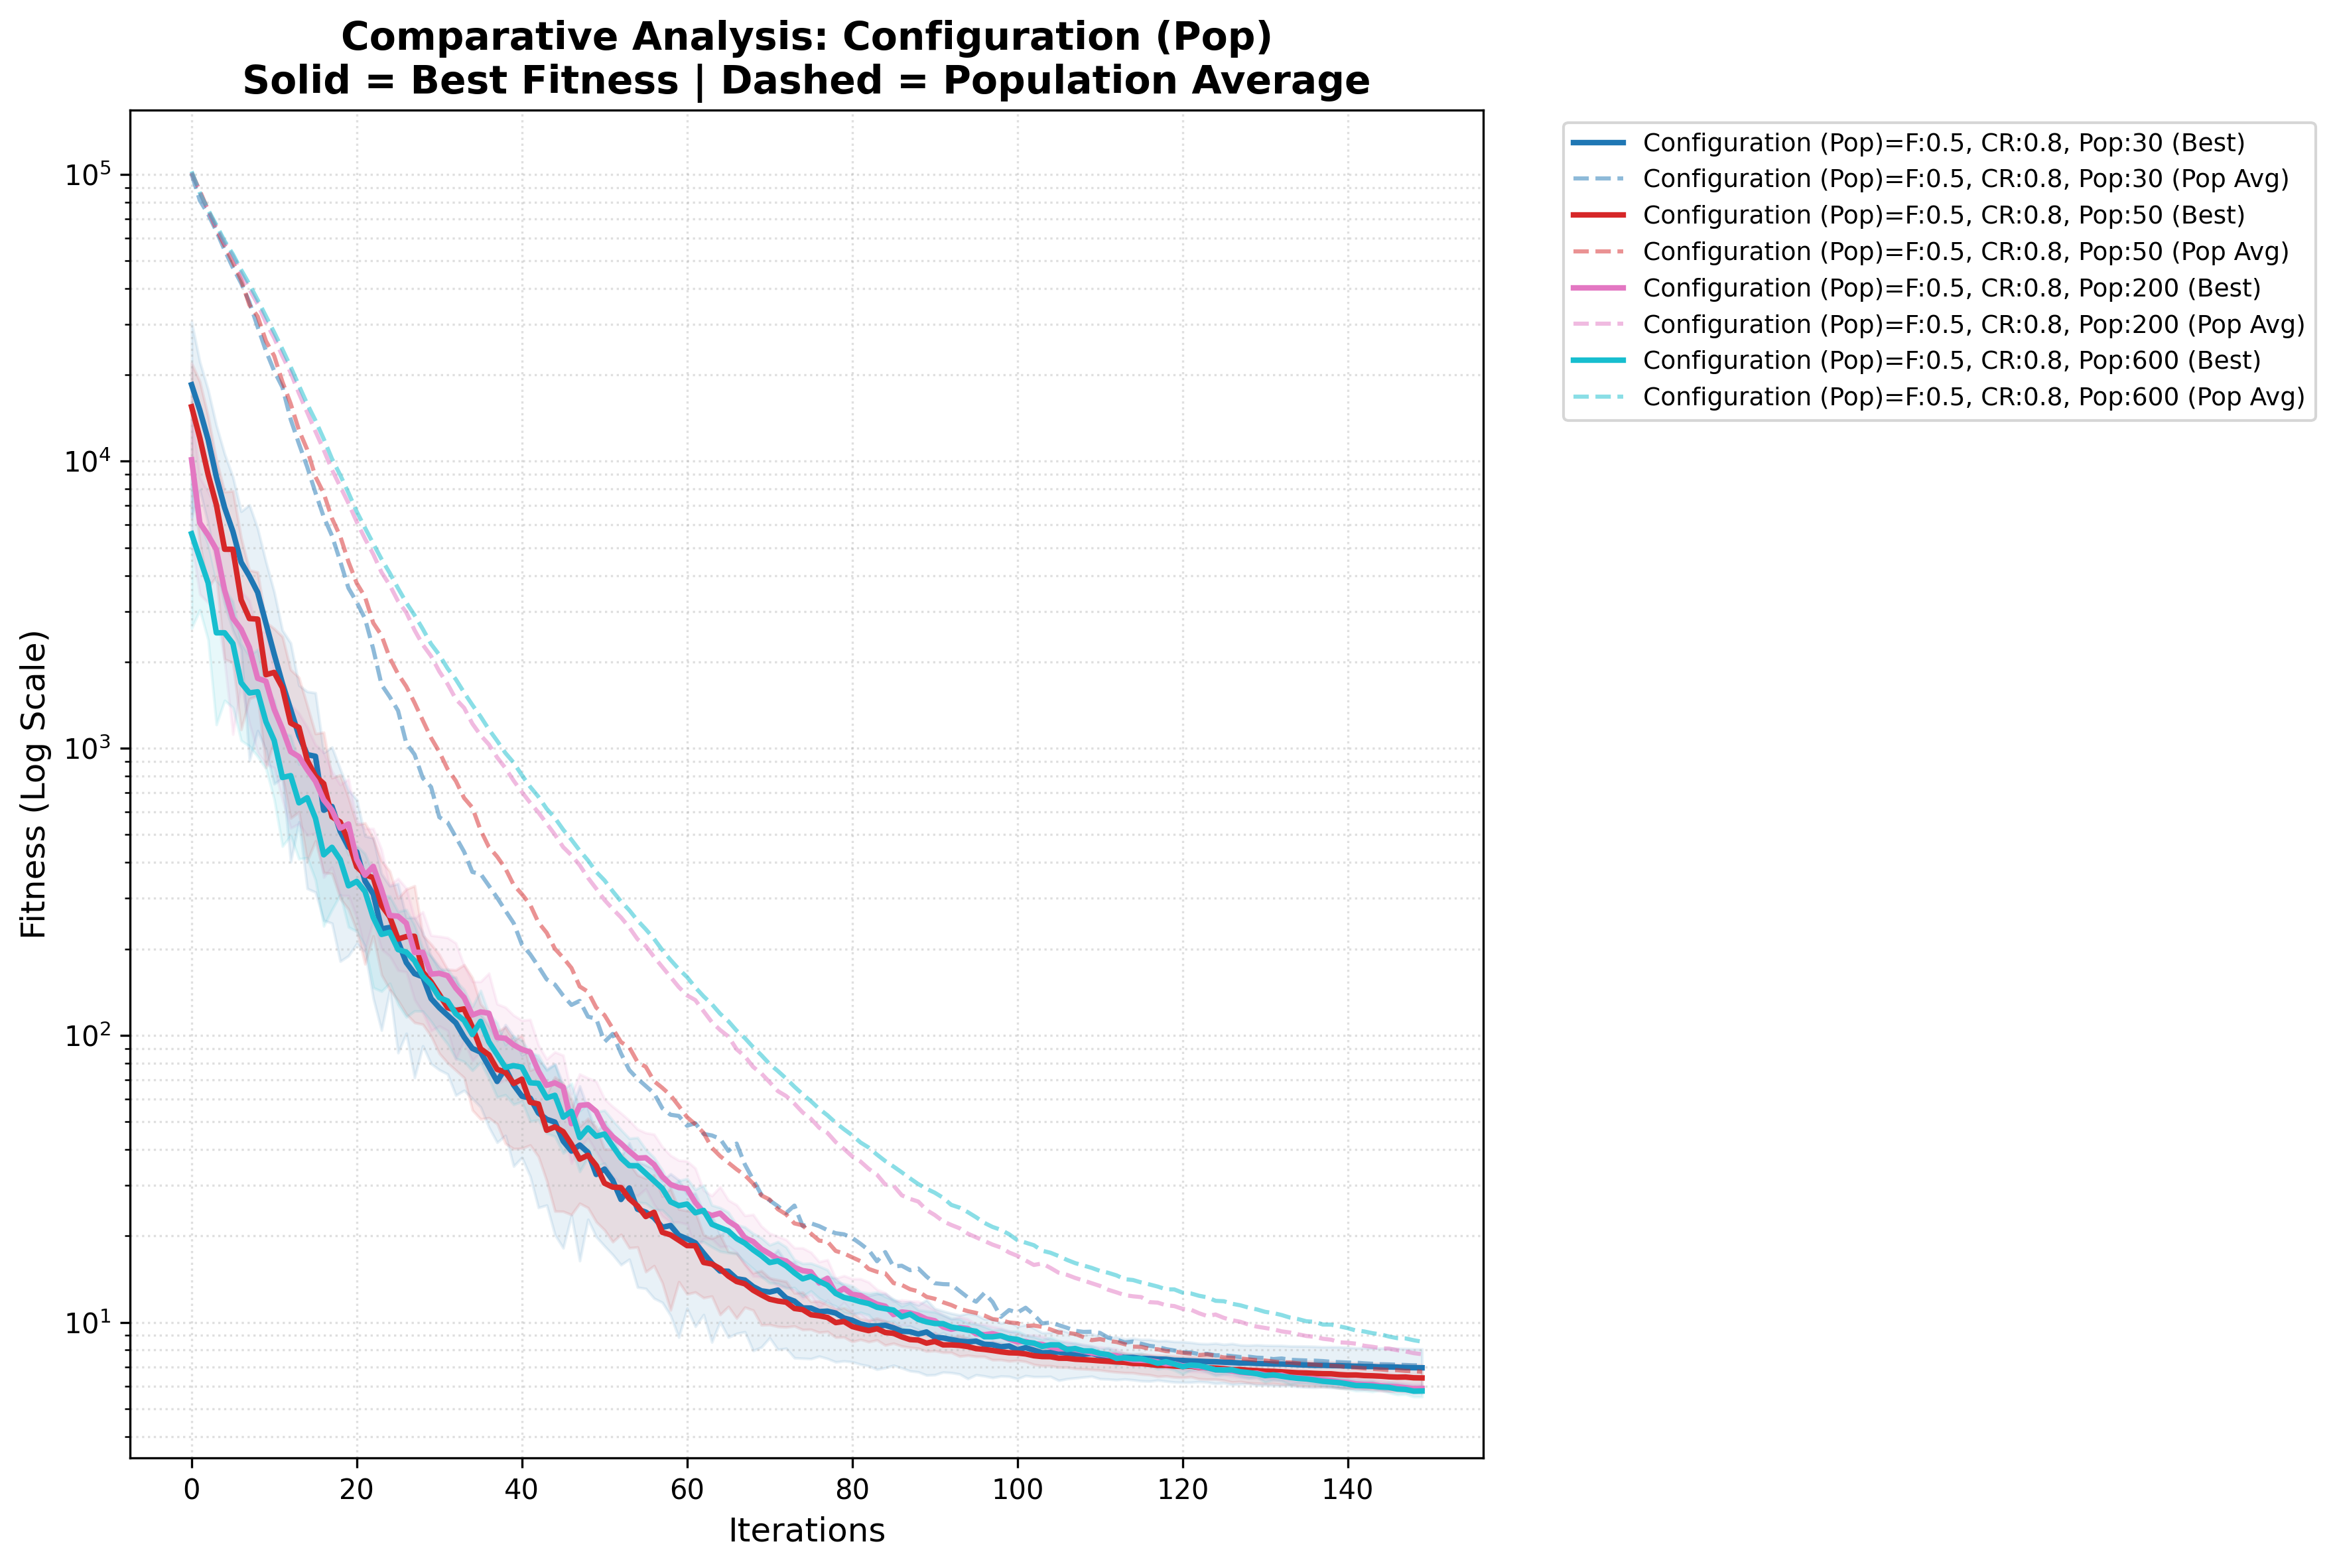
\includegraphics[width=1\linewidth]{comparativa_final_de_rosenbrock_pop.png}
            \caption{Results of the experiments based on population}
            \label{fig:placeholder}
        \end{figure}
        
        Here we can appreciate how, as happened with PSO, the configurations with more populations
         tend to have a higher average of population average.
        
        \item \textbf{Number of Iterations}
        
            The results of the different number of iterations were the following:

        \begin{table}[H]
        \centering
        \begin{tabular}{c c c c}
        \hline
        Iterations & Avg Fit & Min Fit & Std Dev \\
        \hline
        150 & 5.718332 & 5.262399 & 0.187409 \\
        300 & 2.034989 & 1.606199 & 0.240675 \\
        600 & 0.001277 & 0.000460 & 0.000714 \\
        \hline
        \end{tabular}
        \caption{Results DE – Rosenbrock 10D}
        \end{table}
       
        Here we can appreciate how the difference between iterations is also striking, achieving really low values with 600 iterations, 
        although it is not as exaggerated as with Griewank. This phenomenon was to be expected, as Rosenbrock is a harder function, it is more difficult, even for strong algorithms like DE,
        to find the optimal solution.

        The following graph gives us a better understanding of what's happening:
        \begin{figure}[H]
            \centering
            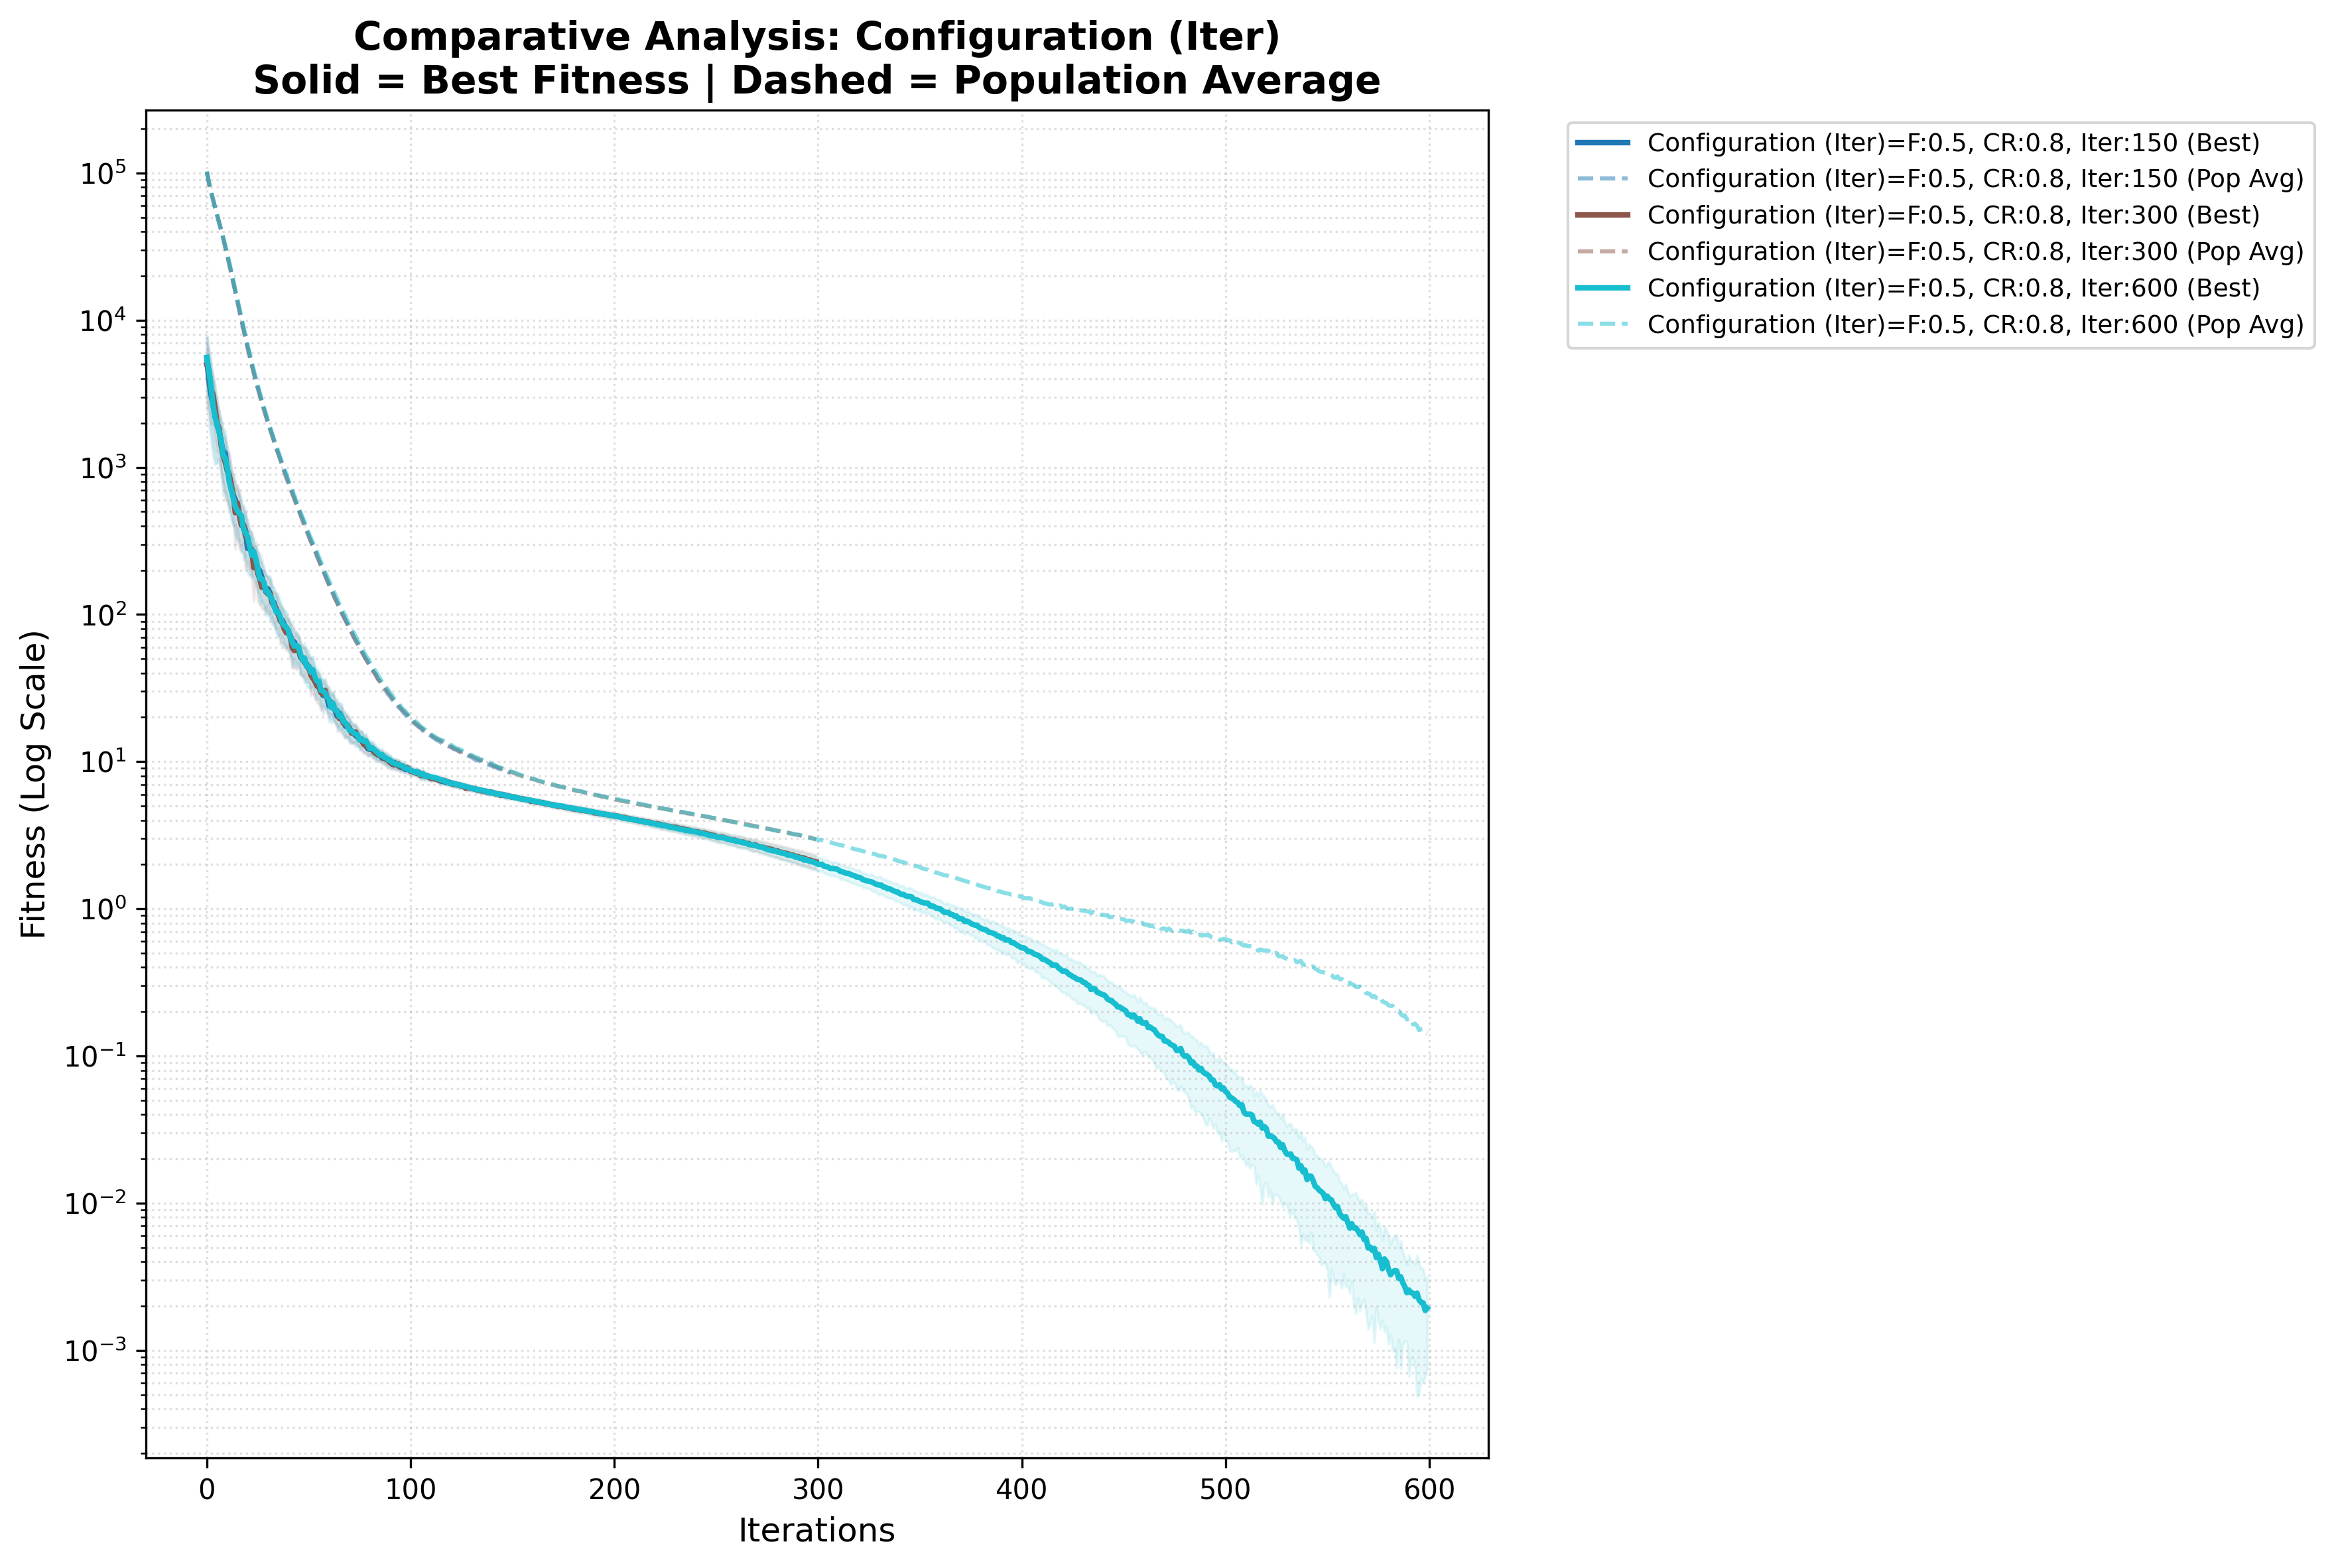
\includegraphics[width=1\linewidth]{comparativa_final_de_rosenbrock_iter.png}
            \caption{Results of the experiments based on iterations}
            \label{fig:placeholder}
        \end{figure}
        We can see the big drop in fitness, but at the same time it is not as sudden as with Griewank, it is more gradual due to the augmented difficulty.
        This is also reflected with the average of population average, in this case it does not drop vertically as with Griewank, meaning the majority of the individuals are still finding the good solutions, but not the best ones.
    \end{itemize}    


\subsubsection{Conclusions on DE}

% With differential evolution, we observed a robust and adaptive optimization process, particularly well-suited for complex landscapes like Rosenbrock. The experiments highlighted several key findings:

% First, the choice of parameters had a decisive impact on performance. For Rosenbrock, the best results were consistently achieved with a moderate mutation factor ($F=0.5$) and a high crossover rate ($CR=0.9$), underscoring the importance of coordinated changes across dimensions in navigating the function's narrow valley. This contrasts with the Griewank function, where lower $CR$ values were more effective, reflecting the different natures of the two landscapes.

% Second, while increasing the population size led to gradual improvements, the effect was less pronounced than in PSO. This suggests that DE's mutation and crossover mechanisms are inherently effective at maintaining diversity, reducing the need for very large populations to avoid premature convergence.

% Third, the number of iterations played a critical role in solution quality. With 600 iterations, DE was able to approach the global optimum on Rosenbrock, achieving extremely low minimum fitness values. This demonstrates the algorithm's capacity for fine-tuning and persistent improvement, especially in unimodal or highly structured search spaces.

% Overall, DE proved to be a highly competitive algorithm, capable of outperforming PSO in certain scenarios, particularly when variable interdependencies are significant. Its adaptive search dynamics and efficient use of population diversity make it a strong choice for continuous optimization problems where both exploration and exploitation are essential.


With differential evolution, we observed great adaptativity and robustness, especially in the Rosenbrock function, which is a more complex landscape. The choice of parameters had a significant impact on performance, with moderate mutation and high crossover rates yielding the best results for Rosenbrock, while lower crossover rates were more effective for Griewank. Increasing population size led to improvements, but the effect was less pronounced than in PSO, suggesting that DE's mechanisms maintain diversity effectively. The number of iterations was critical, with 600 iterations allowing DE to approach the global optimum on Rosenbrock. Overall, DE proved to be a highly competitive algorithm, particularly when variable interdependencies are significant.
\newpage

\subsection{Comparative Analysis}
\subsubsection{PSO vs DE}
% When comparing both algorithms, we can see that DE generally outperformed PSO in both functions, achieving better average and minimum fitness values. 
% This is likely due to DE's more effective exploration and exploitation mechanisms, that assist it in navigating complex search spaces more efficiently. 
% In particular, DE's ability to escape local minimums and fine-tune solutions 
% contributed to its superior performance, especially in the Rosenbrock function where variable interdependencies 
% are significant. PSO, while still effective, struggled more with local minimums and required careful parameter tuning 
% to achieve competitive results.

When comparing both algorithms, we can see that DE generally outperformed PSO in 
both functions, achieving better average and minimum fitness values.

\begin{table}[H]
\centering
\begin{tabular}{c c c c c}
\hline
\textbf{Function} & \textbf{Algorithm} & \textbf{Best Avg Fit} & \textbf{Best Min Fit} & \textbf{Best Std Dev} \\
\hline
\multirow{2}{*}{Griewank 10D} 
& PSO & 0.072795 & 0.019693 & 0.024755 \\
& DE & 3.70e-18 & 0.000000 & 1.99e-17 \\
\hline
\multirow{2}{*}{Rosenbrock 10D} 
& PSO & 1.648496 & 0.000239 & 0.834917 \\
& DE & 0.001277 & 0.000460 & 0.000714 \\
\hline
\end{tabular}
\caption{Best results comparison between PSO and DE}
\end{table}

This is likely due to DE's more effective exploration and exploitation mechanisms 
through its mutation and crossover operators. In particular:

\begin{itemize}
\item \textbf{Griewank:} DE achieved near-perfect results (3.70e-18) compared to PSO's 
0.072795. This demonstrates DE's superior ability to escape the many local minima 
of this multimodal function through its difference vector mutation mechanism.

\item \textbf{Rosenbrock:} DE also outperformed PSO (0.001277 vs 1.648496 average), 
though the gap is smaller. DE's high crossover rate (CR=0.9) allowed coordinated 
changes across interdependent variables, crucial for navigating the narrow valley.
\end{itemize}

\paragraph{Key Differences Observed:}
\begin{enumerate}
\item \textbf{Convergence Pattern:} PSO shows rapid initial convergence but often 
plateaus early. DE shows slower initial progress but continues improving throughout 
all iterations, especially visible in the 300-600 iteration range.

\item \textbf{Parameter Sensitivity:} PSO was more sensitive to parameter changes, 
particularly the inertia weight $w$. DE showed more robust performance across 
different $F$ and $CR$ combinations.

\item \textbf{Population Impact:} Both algorithms benefited from larger populations, 
but PSO showed more dramatic improvements, suggesting it relies more on swarm 
diversity than DE does.
\end{enumerate}
\subsubsection{Comparison with Genetic Algorithm (GA)}
To contextualize the performance of PSO and DE, we compare our results with those obtained from Genetic Algorithm experiments conducted in a previous assignment using the same benchmark functions. It's important to note some methodological differences: the GA experiments used 4-dimensional Rosenbrock while our PSO/DE experiments used 10-dimensional versions, and GA tested both binary and real coding while PSO/DE operate naturally in continuous space.

\begin{table}[H]
\centering
\resizebox{\textwidth}{!}{%
\begin{tabular}{l c c c c}
\hline
\textbf{Algorithm} & \textbf{Configuration} & \textbf{Best Avg Fitness} & \textbf{Best Std Dev} \\
\hline
GA (Real) & Pop 1000, 4D & 0.506016 &  0.126724 \\
PSO & Pop 600, 10D & 1.648496 &  0.834917 \\
DE & Pop 50, Iter 600, 10D & 0.001277 & 0.000714 \\
\hline
\end{tabular}
}
\caption{Performance comparison on Rosenbrock function.}
\end{table}


We can appreciate how Differential Evolution demonstrated clear superiority on the Rosenbrock function, achieving an average fitness of 0.001277 despite operating in 10 dimensions compared to GA's 4 dimensions. 
This result can be attributed to DE's difference-vector mutation mechanism, which naturally coordinates changes across interdependent variables through its high crossover rate (CR=0.9), thus allowing the algorithm to follow Rosenbrock's valley effectively.

Genetic Algorithms with real coding achieved competitive results (0.506016) but required substantially larger populations (1000 individuals) to maintain sufficient diversity.

On the other hand, Particle Swarm Optimization struggled most significantly (1.648496 average), requiring both large populations (600) and many iterations (600) without matching competitor performance. 
This can be explained by its tencency to overshoot the narrow valley. 
With this we can conclude that PSO's strength lies in implementation simplicity rather than raw optimization power for this problem type.


Regarding convergence behavior, DE showed sustained improvement throughout all iterations with dramatic late-stage refinement (iterations 300-600), while PSO plateaued prematurely and GA maintained steadier but slower progress. 

In conclusion, for continuous optimization problems with variable interdependencies like Rosenbrock, Differential Evolution provides the best balance of performance, parameter simplicity, and robustness. GA remains valuable for discrete representations, while PSO requires careful tuning to achieve competitive results on complex landscapes.

\section{Problem 2: Travelling Salesman Problem (TSP)}
For the second problem of this assignment, our objective is to test the PSO algorithm on the Travelling Salesman Problem (TSP), which is a well-known combinatorial optimization problem. The TSP asks for the shortest possible route that visits a set of cities and returns to the origin city.

We will make use of the already implemented PSO-TSP function from the scikit-opt library, 
and we will compare our results to the Genetic Algorithm (GA) that we implemented in a previous assignment.

Our objective is to observe if we can achieve the minimum distance of 7542, which is the known optimal solution for the berlin52 TSP instance, and to compare the performance of PSO with GA in terms of solution quality and computational time.

\subsection{PSO for TSP}
\subsubsection{Parameter Tuning}
While looking at the code of the PSO-TSP function, we discovered that it did not make use of the inertia weight $w$ or the $c1$ and $c2$ parameters, so the only parameters we could tune were the population size and the number of iterations.
Then, we decided to set an iteration number of 2000 to give the algorithm enough time to find good solutions (and because it was the number set in the last assignment), and we focused on tuning the population size, testing the following values: 50, 100 and 200.
We also set the number of runs to 10, it was low but this problem required a lot of time to run, and we wanted to be able to test different configurations in a reasonable amount of time.

\paragraph{Population size}

The results of the different population sizes were the following:
\begin{table}[H]
\centering
\begin{tabular}{c c c c c c c}
\hline
\textbf{Pop} & \textbf{Avg Fit} & \textbf{Min Fit} & \textbf{Std Dev} & \textbf{Time/Round} & \textbf{Avg Error \%} & \textbf{Min Error \%} \\
\hline
50  & 8154.5 & 7764.0 & 252.625909 & 7.603829  & 8.121188 & 2.943516 \\
100 & 8146.5 & 7846.0 & 227.869809 & 13.515571 & 8.015115 & 4.030761 \\
200 & 7776.2 & 7542.0 & 234.131074 & 26.246325 & 3.105277 & 0.000000 \\
\hline
\end{tabular}
\caption{PSO experiments on berlin52}
\end{table}

After these results we observe how we were able to achieve the optimal solution of 7542 with a population of 200, which is a great result, and it shows us that PSO can be effective for solving TSP instances when given enough population diversity.
We can also see how the average fitness and the minimum fitness improved as we increased the population size, which is consistent with our previous observations in the continuous optimization problems, where a larger population allowed the algorithm to explore more of the search space and find better solutions.
The computational time also increased with the population size, which is expected, but it is still reasonable.

In the following graph we can see the behaviour of the algorithm with different population sizes:
\begin{figure}[H]
    \centering
    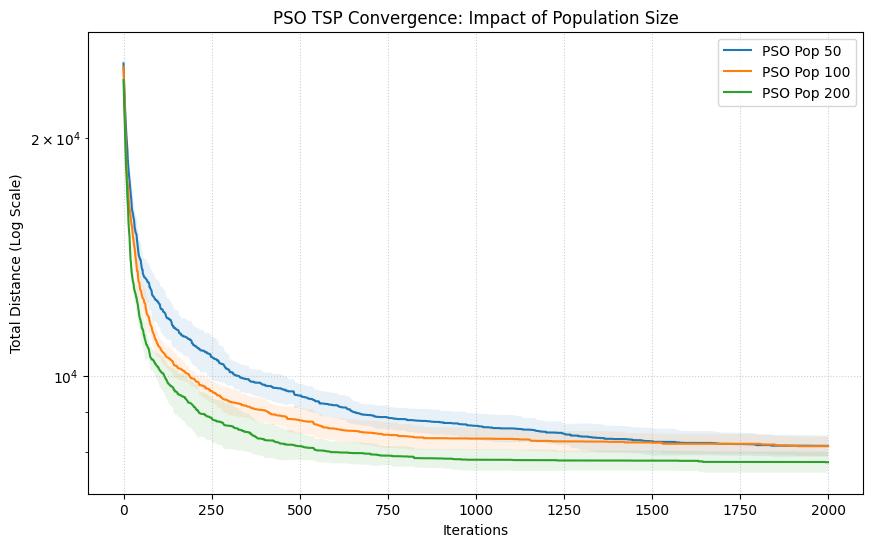
\includegraphics[width=1\linewidth]{comparativa_final_pso_tsp_pop.png}
    \caption{Results of the experiments based on population size for PSO on TSP.}
    \label{fig:placeholder}
\end{figure}
We can see how the configuration with 200 individuals is consistently better than the rest, and it is the only one that was able to achieve the optimal solution, which is represented by the horizontal line at 7542.
In fact, testing with a large number of iterations (2000) already saves us the specific iteration analysis, as we can see the behaviour of the 
configurations at each point of the iterations. On iteration 1000, the configuration with 200 individuals was already capable of achieving the optimal solution, and surprisingly,
the configuration with 50 individuals actually overtook the one with 100, probably due to stochastic effects.

\subsection{GA vs PSO}
The architecture of the GA that we are going to compare with was based on the best configuration we found in the previous assignment, which had a tournament size of 3 and a mutation rate of 1.0.

Its results were the following:
\begin{table}[H]
\centering
\begin{tabular}{c c c c c c c}
\hline
\textbf{Pop} & \textbf{Avg Fit} & \textbf{Min Fit} & \textbf{Std Dev} & \textbf{Time/Round} & \textbf{Avg Error \%} & \textbf{Min Error \%} \\
\hline
   50  & 8095.2 &  7618 & 300.519151 & 5.061666 & 7.334924 & 1.007690 \\
  100 & 8159.5 &  7731 & 217.658563 & 10.385853 & 8.187483 & 2.505967 \\
 200 & 8039.3 &  7542 & 239.275594 & 20.406382 & 6.593742 & 0.000000 \\
\hline
\end{tabular}
\caption{PSO experiments on berlin52}
\end{table}

Now with this data we can make several observations. Firstly, both were able to found the optimum with a population
of 200 but PSO had a better average performance. PSO's average error (3.11\%) 
was half of GA's (6.59\%), it was more consistent.
Secondly, GA is computationally faster, exactly 22\% faster 
than PSO, which is expected given the simpler operations in GA compared to the velocity and position updates in PSO.
Finally, we could observe the critical role of population size in both algorithms, confirming that TSP needs diversity.

\subsubsection{Which Method to Prefer?}

Based on our experiments, we could say that our preference would be determined by the type of the problem we're encountering.
Both PSO and GA proved capable of reaching the optimal solution under sufficiently large populations and iteration counts, but they offer different advantages:
 PSO delivered more consistent solution quality with roughly half the average error of GA, 
 while GA was significantly faster and benefits from a natural permutation‑based encoding and well‑established crossover operators tailored to TSP.

 Overall, if we were to choose one method we would slighly prefer GA for TSP because it is able to achieve the same optimal solution as PSO but with a much lower computational time, and because of its natural suitability for combinatorial problems.
\end{document}
